
This chapter approaches neuroscience from the point of view that there are
clearly functional connections between neurons in the same region of the brain and
that these connections could possibly illuminate the function of the region.  Complex network theory, a branch 
of mathematics closely related to graph theory, appeared as though it could be useful. Complex network theory differs from 
graph theory in that it focuses on the traits that networks tend to have when they evolve in real life, rather than focusing on purely random networks.  
The main difference between these would be the connectivity profile of the 
network; in graph theory connections are usually spread somewhat uniformly 
through the graph, whereas in Network Theory it is  expected that communities would form \citep{Newman2010a}.

A mathematical network is simply a collection of nodes and links between
these nodes.  An \emph{undirected network} with $n$ nodes can be
completely described by the adjacency matrix $A_{ij}$ where $A_{ij} =
1$ if nodes $i$ and $j$ are connected, and is equal to zero otherwise. In this 
case $A_{ij} = A_{ji}$ since two nodes are either connected or
not.  If matrix entries $A_{ij}$ are permitted to take values other than one and zero
then that is called a \emph{weighted} network, and if the matrix is not symmetric; it is called a \emph{directed} network, where $A_{ij} = 1$ if there 
is an arrow pointing from node $j$ to node $i$.   Binary undirected networks form the bulk of the literature, and so the theory is richer
in this case. A reason for this could be that networks such as friend networks \citep{Zachary1977a} would typically not be directed as friendship is typically mutual.

A particularly interesting part of network theory that could be useful for
neuroscience is clustering, and algorithms to maximise the community structure of the communities.  The main focus is on a measure known as the
\emph{modularity} \citep{NewmanGirvan2004a}.

\section{Modularity}

The \emph{modularity} is a measure of a given clustering of a network,  it is defined to measure how much more prominent
intra-cluster links are than inter-cluster links in a given
clustering. The modularity then, as a measure of the given clustering, measures how much community structure is seen in the network.  It was introduced by Newman and Girvan \citet{NewmanGirvan2004a} in one form, then Newman \citet{Newman2006b, Newman2006a} derived another form using the configuration model for graphs \citep{BenderCanfield1978a,Bollobas1980a}.


\begin{figure}[htb]
  \centering
  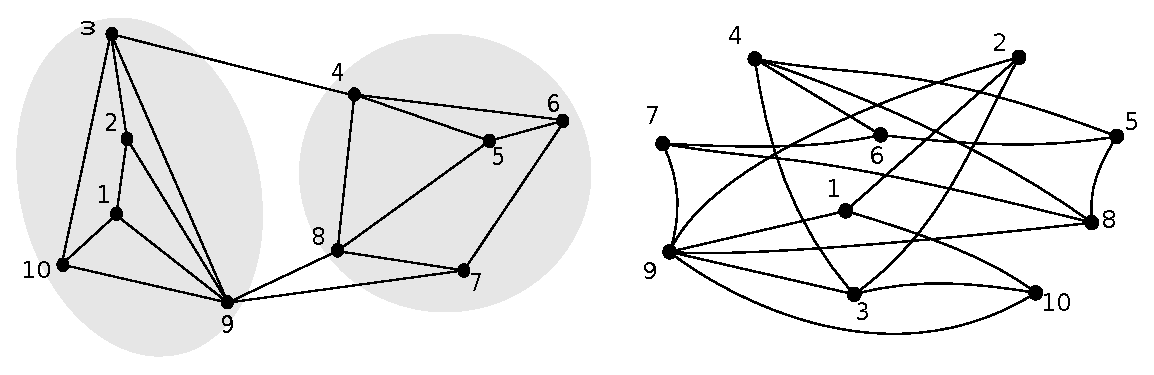
\includegraphics[width=0.9\textwidth]{networkcvsnc.eps}
  \bigskip
  \rule{35em}{0.5pt}
  \caption{The advantage to clustering a network correctly is seen here.  Both 
    of these networks have the same nodes and links, and so are the same 
    network, but they look vastly different because the diagram on the left 
    has been clustered to maximise modularity.}
  \label{netclus}
\end{figure}

The modularity is a measure of a clustering of a network that assesses 
how much more community structure there is in the network than there would be 
in a random network with similar properties.  In \citep{Newman2006b,Newman2006a} the modularity is derived as follows. The modularity is defined to be the difference between actual links within clusters and the expected number of links.  Summing over all nodes within a cluster, $g$, this is:
\begin{equation}
(\text{Links in }g) - (\text{Expected links in }g) = \sum_{i,j \in g}  A_{ij} - \sum_{i,j \in g} P_{ij} 
\end{equation}
where $P_{ij}$ is the 
probability of a link between nodes $i$ and $j$. Then, if $g_i$ is the 
community to which node $i$ belongs, the modularity $Q$ can be described:

\begin{equation}
Q = \frac{1}{2m}\sum_{i,j}[A_{ij} - P_{ij}]\delta(g_i,g_j)
\end{equation}
where $\delta$ is the Kronecker delta, so $\delta(g_i,g_j)=1$ if nodes 
$i$ and $j$ are in the same cluster, and zero otherwise. $m$ is the total 
number of links in the network, and so $1/2m$ is just a normalising 
factor.  The modularity of a cluster is then the number of edges within a 
cluster minus the expected number of edges.

\citet{Newman2006b,Newman2006a} calculates the probability of a link between nodes in the configuration model.  In undirected networks, 
clearly the probabilities should be symmetric, $P_{ij} = P_{ji}$.  Then, the expected number of links across the whole network should equal the total number of links.   That is, $\sum_{i,j}[A_{ij} - P_{ij}] = 0$, and,
\begin{equation}
\sum_{i,j}P_{ij} = \sum_{i,j} A_{ij} = 2m,
\end{equation}
where $m$, as before, is the total number of edges in the network, so if the 
degree of node $i$ is $k_i$, then
\begin{equation}
m = \frac{1}{2}\sum_i k_i = \frac{1}{2}\sum_{i,j} A_{ij}.
\end{equation}

At this point, there is some choice as to how similar the random network should be to the network itself.  One could suppose that each node 
in the random network has degree equal to the average degree of the 
network, but this ignores local structure in the network.  Instead, it is supposed that 
the random network should keep the same degree for all nodes, and so the network can be treated as an instance of the \emph{configuration model} \citep{BenderCanfield1978a, Bollobas1980a}.  So, the expected 
degree of each vertex is equal to the actual degree of the vertex:
\begin{equation}
\sum_j P_{ij} = k_i.
\label{probki}
\end{equation}

If it is supposed that beyond the degree distribution that edges are placed at random, 
then the probability of two nodes connecting depends on their 
degrees. Supposing the probabilities for each end of a single edge is independent, which is a reasonable assumption in a large network \citep{Newman2010a}, where all the degrees are small 
relative to the total number of edges, get that $P_{ij} = f(k_i)f(k_j)$ for 
some function $f$ on their degrees.  Then, by equation \ref{probki}, get
\begin{equation}
\sum_{j=1}^{n}P_{ij} = \sum_{j=1}^n f(k_i)f(k_j) = f(k_i)\left[\sum_{j=1}^n f(k_j)\right]=k_i,
\end{equation}
so $f(k_i) = Ck_i$, for some constant $C$, and we get
\begin{equation}
2m = \sum_{i,j}P_{ij} = C^2\sum_{i,j}k_ik_j = (2mC)^2,
\end{equation}
so, $C = 1/\sqrt{2m}$ which gives the probability $P_{ij}$ as
\begin{equation}
P_{ij} = \frac{k_i k_j}{2m},
\end{equation}
and the modularity is
\begin{equation}\label{NewMod}
Q= \frac{1}{2m}\sum_{i,j} \left(A_{ij} -
\frac{k_ik_j}{2m}\right)\delta(g_i,g_j).
\end{equation}

The modularity gives values between $-1/2$ and $1$ for any clustering.  Since it is known that not 
dividing the network into separate clusters gives a modularity of zero, this 
gives us a lower bound for ``good'' clusterings.

The benefit of finding a good clustering can be seen in figure \ref{netclus}; 
a good clustering can reveal what the nature of the network is, rather than it 
being a mess of nodes and links.  While the modularity itself is a measure of a 
given clustering of a network, the maximum modularity is a property of the 
network itself, which can tell much about the inherent community structure of the 
network. To actually determine what clustering will give the maximum modularity an exhaustive search would be required, which becomes unfeasible for networks of even  a moderate size, as the number of potential clusterings is huge. Therefore, clustering algorithms are needed to 
maximise the modularity.



\section{Newman's eigenvalue algorithm}

In \citep{Newman2006a,Newman2006b} Newman noted that if it was supposed that the network was 
split into two clusters, then the modularity could be redefined in terms of a
quadratic form.  Defining a vector $s$, which keeps track of the
split,
\begin{equation}
s_i = \left\{ \begin{array}{ll} 1 & \mbox{if node $i$ in cluster 1}
  \\ -1 & \mbox{if node $i$ in cluster 2}\end{array} \right.
\end{equation}
These vectors $s_i$ then contain the exact same information as the $n\times 2$ matrix $\delta (g_i,g_j)$, so $\delta (g_i,g_j) $ can be factored by:
\begin{equation}
\delta (g_i,g_j) = \frac{1}{2} \left( s_i s_j + 1 \right)
\end{equation}
Then, the modularity is redefined as:
\begin{eqnarray} \label{ssMod}
Q & = & \frac{1}{2m}\sum_{i,j} \left(A_{ij} - \frac{k_ik_j}{2m}\right)\frac{1}{2}(s_is_j + 1)\cr
& = &\frac{1}{4m}\sum_{i,j} \left(A_{ij} - \frac{k_ik_j}{2m}\right)s_is_j,
\end{eqnarray}
Let $\mathbf{B}$ be a matrix where 
$B_{ij} = A_{ij} - k_ik_j/2m$, called the \emph{modularity matrix}, 
then equation \ref{ssMod} becomes:
\begin{equation}
Q = \frac{1}{4m}{\bf s^tBs}
\end{equation}

Now, since $\mathbf{B}$ is an $n\times n$ symmetric matrix, it has $n$ real eigenvalues $\lambda_i$, with corresponding
eigenvectors $u_i$.  Ordering the $\lambda_i$ so that $
\lambda_1 \geq \lambda_2 \geq \ldots \geq \lambda_n$, then write 
\begin{equation}
{\bf s} = a_1{\bf u_1}+ \ldots + a_n{\bf u_n}.
\end{equation}


The equation for the modularity becomes
\begin{eqnarray}
Q & = & \frac{1}{4m} \sum_{i} a_i{\bf u}_i^t{\bf B}\sum_ja_j{\bf u}_j\cr
& = & \frac{1}{4m} \sum_i \lambda_i ({\bf u}_i^{\bf t}.{\bf s})^2
\end{eqnarray}
so, the positivity of the modularity depends completely on the $\lambda_i$, in 
particular the most positive eigenvalue $\lambda_1$.  This means that to 
maximise the modularity the ``split vector'' $\mathbf{s}$ ought to be 
as close to the first eigenvector $\mathbf{u}_1$ as possible. To do this, 
choose $\mathbf{s}$ as follows:

\begin{equation}
s_i =\left\{ \begin{array}{ll} 1 & \mbox{if } u_{1_i}>0 \\
-1 & \mbox{if } u_{1_i}\leq0 \end{array} \right.
\end{equation}

This gives a clustering of the network into two smaller clusters. Of course, 
this split is not strictly in the direction of $\lambda_1$, but it is the best 
possible estimate\footnote{In fact, it has been noted from well-known networks, 
such as Zachary's karate club \citep{Zachary1977a} that the absolute value of 
the $i$th entry of $\mathbf{u}_1$ gives a good indication of the ``strength'' 
of the membership of node $i$ to its cluster \citep{Newman2006a}.}, given two 
clusters. If the modularity of the split is not positive, then reject the 
split and say that the best clustering is to leave the network as it is.  
Similarly, if the first eigenvalue $\lambda_1 = 0$ then say that the best 
clustering is to leave the network undivided, as it is known that the modularity 
matrix $\mathbf{B}$ always has a zero eigenvalue, with eigenvector 
$\mathbf{u} = ( 1,1, \ldots, 1)$, which corresponds to no split of the network.

With the network split into two smaller clusters, the next
question is how to split the network further.  Newman \citep{Newman2006a} recommends looking at the clusters
one-by-one and splitting them until it gives no benefit to the modularity
of the overall clustering.  One could naively just look at the
adjacency matrix of the cluster itself, and form the 
corresponding modularity matrix, but this ignores the connectivity of the
overall network.  That method could inadvertently split the subgraph into communities 
which would make sense within the cluster, but would ignore the connections 
from outside the cluster. Instead, the original modularity 
matrix $\mathbf{B}$ is used to calculate what difference a split of the subgraph would 
make to the modularity.

Call the cluster of nodes $g$ and the \emph{modularity contribution} $\Delta Q$ of a 
split of $g$ is:

\begin{equation}
\Delta Q  =  \frac{1}{2m} \left[ \frac{1}{2}\sum_{i,j\in g}B_{ij}(s_is_j + 1) - \sum_{i,j \in g} B_{ij} \right].
\end{equation}

This is the term in the modularity of the network that a split $\mathbf{s}$ of 
$g$ would change, minus the modularity of leaving the subgraph $g$ whole.  Thus, a ``subgraph modularity matrix'' $\mathbf{B}^{(g)}$ can be defined:

\begin{samepage}
\begin{eqnarray}
\Delta Q & = & \frac{1}{4m}\left[ \sum_{i,j \in g} B_{ij}s_is_j - \sum_{i,j \in g}B_{ij}\right] \cr
& = & \frac{1}{4m}\sum_{i,j \in g}\left[ B_{ij} - \delta_{ij}\sum_{k \in g} B_{ik}\right]s_is_j \cr
& = & \frac{1}{4m}{\bf s^tB}^{(g)}{\bf s}
\end{eqnarray}
\end{samepage}
and so ${\bf B}^{(g)}$ that takes the value
\begin{equation}
B^{(g)}_{ij} = B_{ij} - \delta_{ij}\sum_{k \in g} B_{ik}
\end{equation}
for labels $i,j$ of nodes in the cluster $g$.

\begin{algorithm}
\caption{This is Newman's eigenvalue algorithm for maximising the modularity of a network.}
\label{algo-split}
\begin{algorithmic}
\STATE Calculate the modularity matrix $\mathbf{B}$, where $B_{ij} = A_{ij} - k_ik_j/2m$
\STATE Find the most positive eigenvalue $\lambda_1$ and its eigenvector $\mathbf{u}_1$
\IF{$\lambda_1 = 0$}
\STATE Stop the algorithm with no split in the network.
\ELSE
\STATE Split network such that node $i$ in first group if $u_{1_{i}} > 0$ and in second group otherwise.
\ENSURE Modularity of split $> 0$
\ENDIF
\FORALL{Subnetworks $g$}
\STATE Calculate $\mathbf{B}^{(g)}$, where $B^{(g)}_{ij} = B_{ij} - \delta_{ij}\sum_{k\in g}B_{ik}$
\STATE Find the most positive eigenvalue $\lambda^{(g)}_1$ of $\mathbf{B}^{(g)}$ and its eigenvector $\mathbf{u}^{(g)}_1$.
\IF{$\lambda^{(g)}_1=0$}
\STATE Subnetwork can split no further.
\ELSE
\STATE Split network such that node $i$ in first group if $u^{(g)}_{1_{i}} > 0$ and in second group otherwise
\ENSURE $\Delta Q > 0$ for split of subnetwork $g$.
\ENDIF
\ENDFOR
\end{algorithmic}
\end{algorithm}

The same approach as before is used, the most
positive eigenvalue of ${\bf B}^{(g)}$ determines the favoured split
${\bf s}$ to maximise $\Delta Q$. ${\bf B}^{(g)}$ still has the
property that each of its rows and sum to zero, so there still is a
zero-eigenvalue that represents no split of the cluster.  This can
now be the stopping criterion for the algorithm; if the most positive eigenvalue is the
zero-eigenvalue say that the subgraph is indivisible and stop
splitting.  However, it should be noted that as the most
positive eigenvalue gets smaller, relative to its negative
eigenvalues, there may be no benefit to the modularity of accepting
such a split.  In this case  check, by calculating $\Delta Q$ for
the proposed split, to see if it is worth continuing splitting the subgraph.
If $\Delta Q \leq 0$ then stop, otherwise continue
splitting the graph.  The algorithm is summarised in algorithm \ref{algo-split}.  

This eigenvalue method for maximising the modularity has shown
remarkably good results \citep{Newman2006a}, despite the apparent drawback of always splitting the 
network/subgraph in two parts.  It is possible split the network into more than two parts initially by using the first $m$ 
eigenvalues and use the $i$th entry of the eigenvectors as coordinates in 
$\mathbf{R}^{m}$ \citep{Humphries2011a}, but this then requires a choice of 
number of clusters.  This may also 
require calculating many more eigenvalues of the large matrix $\mathbf{B}$, 
which can be computationally expensive, rather than calculating a single eigenvalue for smaller and smaller matrices as above.  


\section{New network clustering algorithms}
Using the definition of modularity as defined above in equation \ref{NewMod} to measure the community structure of given clusterings, two new algorithms were developed in the course of this thesis.  They both use complexity algorithms, and so tend to be a lot slower than principled clustering algorithms such as in \citep{Newman2006a} \citep{NewmanGirvan2004a}.

\subsection{Genetic algorithm}
Genetic algorithms have become very popular to solve complex optimisation problems where it is difficult to calculate the gradient of the objective function.  The algorithm is based on the process of Darwinian evolution where successful genes remain in the gene pool and unsuccessful genes die out.  There have been several clustering algorithms proposed which use the genetic algorithm as their framework, such as \citep{Pizzuti2008a}. In this proposed algorithm the genes are simply the clusterings of a given network and the modularity is then the objective function.

The simplicity of a typical genetic algorithm is that it typically only needs a fitness/objective function to evaluate the fitness of solutions.  A typical genetic algorithm is described in algorithm \ref{genal}.

\begin{algorithm}
\caption{An example of a generic genetic algorithm.}
\label{genal}
\begin{algorithmic}
\STATE Generate a random population of $n$ genes $g_i$, set generation to zero.
\WHILE{ Generation $<N$ }
\FORALL{ Genes $g_i$}
\STATE Calculate the fitness of $g_i$.
\ENDFOR
\STATE Breed new population:
\FOR{ $i \in \{ 1,\ldots,n\}$.}
\STATE Choose parents according to goodness-of-fit.
\STATE Generate new gene $\tilde{g_i}$ by crossover of parent genes.
\STATE Mutate $\tilde{g_i}$ with probability $\epsilon$.
\ENDFOR
\FORALL{$g_i$} \STATE $g_i \leftarrow \tilde{g_i}$ \ENDFOR
\ENDWHILE
\end{algorithmic}
\end{algorithm}

To define a genetic algorithm, it is important to define what a solution is, and how the genes crossover and mutate from generation to generation. In this case, a solution is any clustering of the network.  A fitness function is a function on solutions which should typically be non-negative. This can be attained by setting the fitness of any clustering with negative modularity to zero, but since the lower bound is sharp it is better to use the modularity plus $1/2$ as the fitness function, $f$. Then a clustering $g_i$ is chosen as a parent with probability $f(g_i)/(\sum_j f(g_j))$.

It is important to maintain aspects of the ``parent'' genes when breeding the new genes; the number of clusters is a very important aspect of a clustering, so any algorithm must be careful not to simply crossover clusterings by taking their intersection as that would typically increase the number of clusters.  This can be achieved by setting the upper bound for the number of clusters to be the maximum of the numbers of clusters of the parents, or by setting $n_c = \left(n_i f(g_i)+n_j f(g_j)\right)/(f(g_i)+f(g_j))$.

Crossover is defined in this algorithm by randomly choosing a single node in the network according to the degree distribution, and then randomly choose the cluster which contains the node in one of the parents.  Remove all nodes in the chosen cluster from the selection pool, and continue the process.  If the number of clusters reaches the predefined maximum number of clusters and some nodes remain, then the remaining nodes are placed in the closest cluster to them (by path distance).  Mutation is defined by randomly moving a small (~$15\%$) percentage of nodes between clusters in approximately $10\%$ of clusterings.

This algorithm is very computationally expensive for small networks, but scales much better than Newman's eigenvalue algorithm.

\subsection{Simulated annealing}

Another algorithm from complexity theory which has previously been used for finding community structure in networks is \emph{simulated annealing}.  Simulated annealing is an algorithm based on the technique of annealing in metallurgy; annealing happens when a metal is heated and then cooled slowly to increase the size of the crystals in the metal, as the metal finds the lowest energy state as it cools slowly.

Simulated annealing mimics this process to find a solution that minimises an \emph{energy} function, by introducing a \emph{temperature} of sorts to the system. At each temperature level, there is a small change to 

The probability of changing the state of the system is then determined by an \emph{acceptance probability function}, $P(E(s),E(s'),T)$, which depends on the current energy $E(s)$, the potential new energy $E(s')$ and the temperature $T$.  The basic rule of the algorithm is that any change of state that reduces the energy of the system is automatically accepted, and a change of state that increases the energy is accepted with a probability that decreases as $T\rightarrow0$.

The acceptance probability function used also has the property that small increases in energy are more likely to be accepted than big increases in energy, as can be seen:
\begin{equation}
P(E(s),E(s'),T) = \left\{ \begin{array}{ll} 1 & E(s')<E(s) \\ \min(e^{-\frac{E(s')-E(s)}{T}},1) & E(s') \geq E(s) \end{array} \right.
\end{equation}

The solution space for this algorithm was the space of clusterings of a given network $N$.  The ``energy'' function was the modularity with the sign reversed.

It is important for simulated annealing that all moves are small.  With this in mind, the move in this clustering algorithm is simply to select a node at random and move it to either any existing cluster or to form a new cluster from it.  This algorithm was not particularly good at splitting a network to more than two or three clusters, but it did seem to find ``stable'' solutions, eg. in Zachary's karate club network \citep{Zachary1977a} it found the correct split, rather than the clustering which resulted in a slightly higher modularity.


\section{$k$-medoids clustering}
By defining a metric on spike trains, we can tell how close different responses 
are to each other, but there are no ``co-ordinates'' in the metric space which 
would help with clustering responses.  The standard method of clustering 
spike-trains is similar to $k$-means clustering, but since there is no standard 
method for computing a ``mean spike-train'' given a number of spike trains, it 
must be altered slightly.

\begin{figure}[htb]
  \centering
  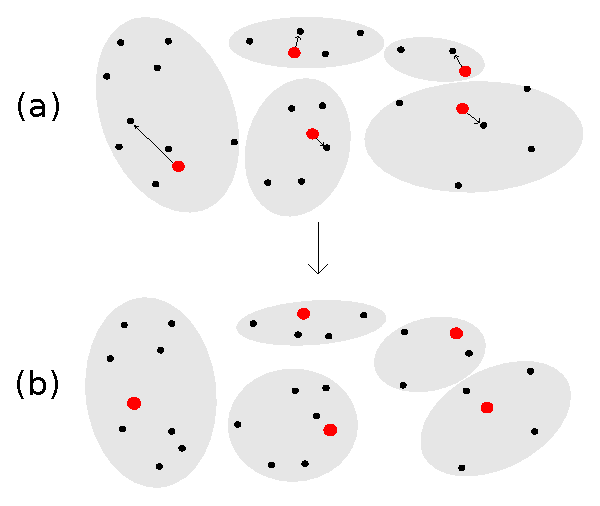
\includegraphics[width=0.6\textwidth]{kmedoids.eps}
  \bigskip
  \rule{35em}{0.5pt}
  \caption{An example of the first step in k-medoids clustering:  (a) Medoids 
    are initially selected at random and the first clustering puts each point 
    in the cluster of the closest medoid. Then we choose the point in the 
    cluster that will give the lowest total distance to other points, and 
    choose that as the new medoid. (b) Finally, we re-cluster each point to go 
    in the cluster of the closest medoid to it.  \label{kmed}}
\end{figure}


For $k$-means clustering, $k$ random points are selected in the space in which 
clustering is occurring, then each point in the space would be in the cluster of 
the closest of these $k$ points to itself.  Then the mean of all 
the points in a cluster is calculated to get a new ``centre'' for the cluster and re-cluster 
each point to the closest of these $k$ means.  This process is repeated until 
the means are stable, which gives a clustering of the points into $k$ clusters.

There is no mean in the metric space of spike-trains, and so  
$k$-means clustering cannot be used.  In \citep{JulienneHoughton2012a} an \emph{average function} is suggested as a possibility to replace the concept of a `mean spike-train', however  the common method is to use $k$-medoids clustering instead.  The algorithm, 
$k$-medoids, begins by choosing $k$ points in the data, called medoids, 
and then  each other point of the data is placed in the cluster of the 
closest (or, least dissimilar) medoid to it.  Then, for each cluster, 
 each point in the cluster is assessed, and the point with 
the least overall distance is chosen as the new medoid. This step is shown in Figure 
\ref{kmed}. These steps are repeated until there is no change in the 
medoids.  This method suits for spike-trains, as the idea of a `mean'
spike-train is not well understood, although, using the van Rossum metric, the average function of Houghton and Julienne is a possible alternative.

There are some downsides to using $k$-medoids, that could possibly be 
improved by using network methods.  The primary disadvantage is that the number of 
 clusters must be selected in advance, and hence implies prior knowledge of the number of different 
stimuli that are presented in a data set.  The next chapter deals with our 
efforts to address this issue.

\section{Clustering responses with modularity}

Here it is proposed that current methods of sorting 
responses could be improved by using the modularity clustering algorithm.  An advantage to such 
a dynamic method could be that responses could be tested without foreknowledge of the stimuli.  This could potentially be an advantage to future dynamic sorting algorithms. Since the algorithm determines when to stop itself, it 
could simply be run to completion.  Such a method could perhaps be used for 
many different data sets, when the number of stimuli was not known, to 
determine the different responses.

The data set introduced in the introduction from \citep{NarayanEtAl2006b} was used, which featured spike trains 
from anesthetized adult male zebra finches as they listened to conspecific 
songs.

A network was formed by first taking the Van-Rossum metric distances between 
each pair of responses, then a threshold value, $\tau$, was chosen for the network 
and the adjacency matrix was calculated as:
\begin{equation}
A^{\tau}_{ij} = \left\{ \begin{array}{ll} 1 & \mbox{if }d(i,j)<\tau \\
0 & \mbox{otherwise}
\end{array}\right. .
\end{equation}

\begin{figure}[h!tb]
  \centering
  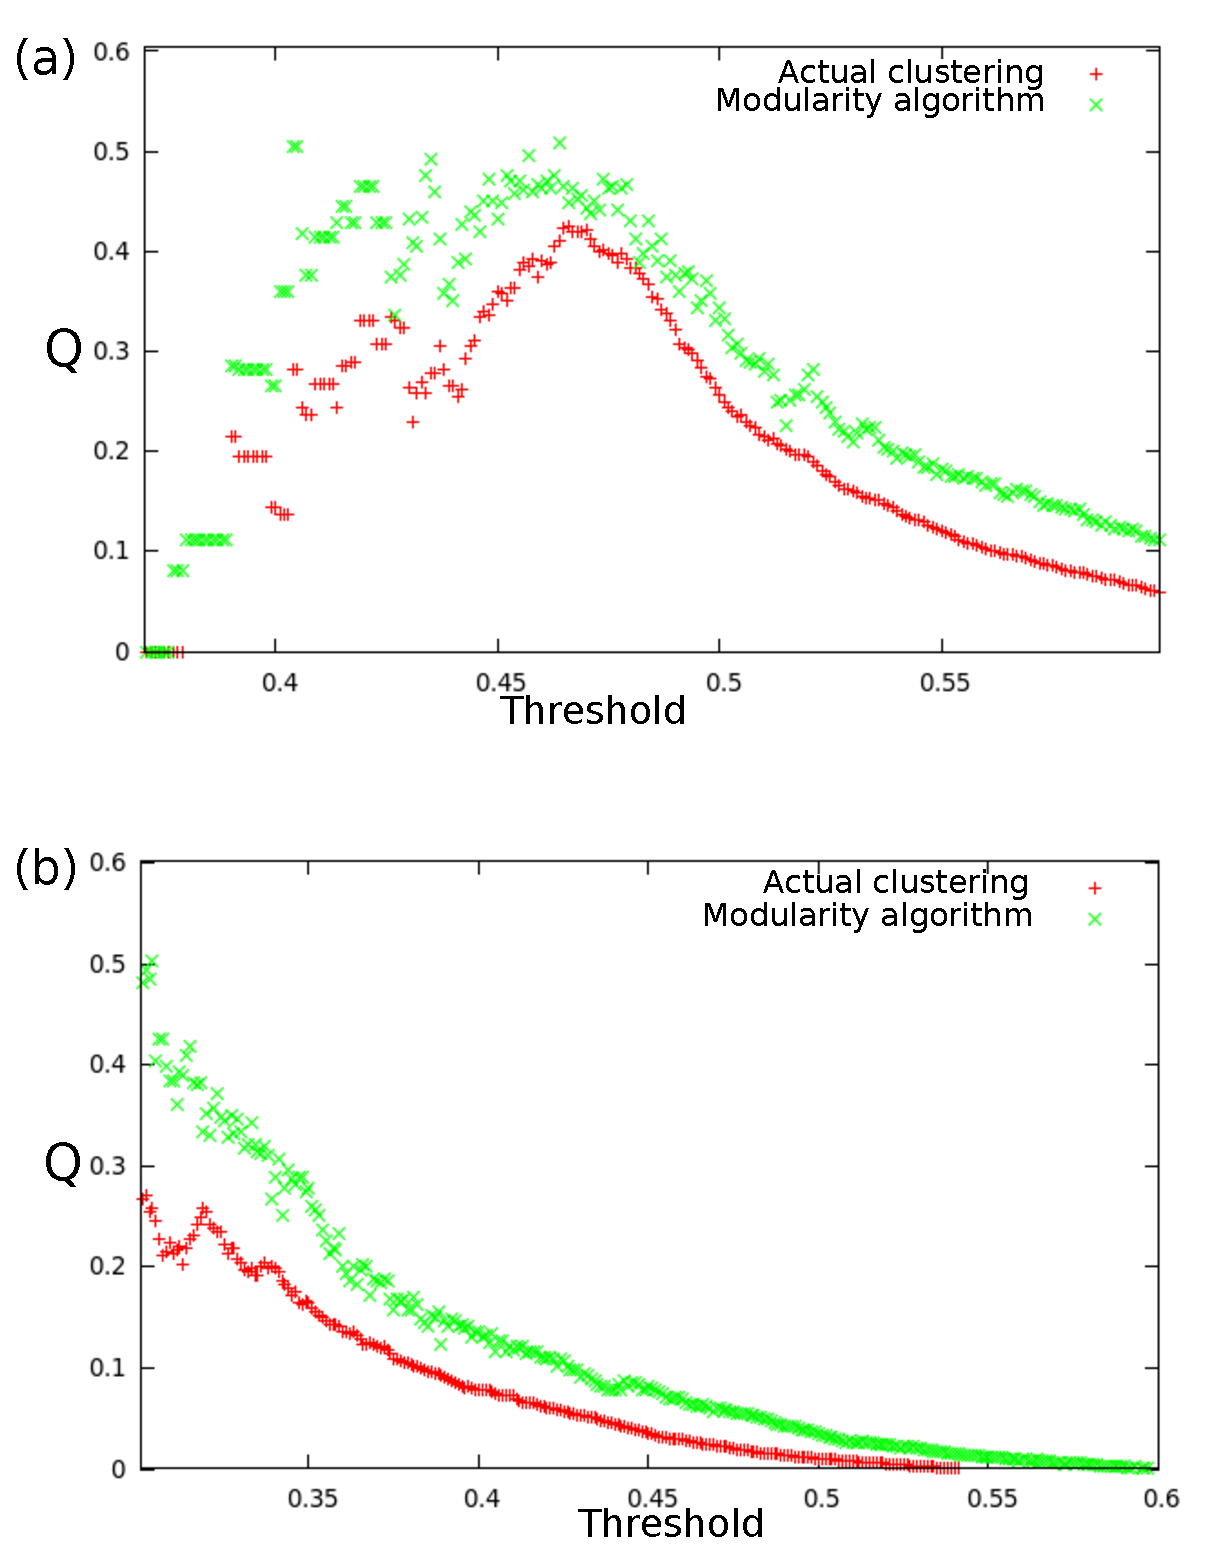
\includegraphics[width=0.5\textwidth]{expresults.eps}
  \rule{35em}{0.5pt}
  \caption{Above is the graph of the modularity versus threshold values
    in two typical cells from the data.  The green crosses represent the 
    modularity of the correct clustering of stimuli; the red plusses represent 
    the maximum modularity, according to the algorithm, of the network.
    Despite there being clear peaks in the modularity graphs, the green 
    consistently outperforms the red for every value of the threshold $\tau$.  
    This seems to imply that network clustering methods are probably not very 
    good for sorting stimuli.  \label{graphs}}
\end{figure}

Once the adjacency matrix was calculated, the algorithm was run to 
maximise modularity for the network.  The maximum van Rossum 
distance, once normalised, between any two trains was one, so the algorithm was run for different 
threshold values $\tau$ between zero and one incrementing $\tau$ by steps of 
size $0.001$.

As seen in Figure \ref{graphs}, the profile of the graph of the maximum 
modularity versus the threshold looked promising, as in nearly all cases it had 
a clear maximum, but unfortunately the clusters of responses bore little 
resemblance to the stimuli, and usually had too few clusters.


The modularity maximisation unfortunately cannot separate the stimuli in these networks. A similar method was used in \citep{Humphries2011a}, where all of the positive eigenvalues were used to 
cluster the responses with more accuracy. This method is 
rather computationally expensive, and uses even the very small positive 
eigenvalues, which themselves may have little effect on the positivity of modularity.  This motivated the attempt to use the clustering method of \citet{Newman2006b}, but it did not perform very well.

The problem with the above method appears to be that there is no natural network formed by the distance matrix of responses to stimuli. The next section introduces a simulated network of neurons, so that there is a definite network structure to investigate.

%
%Once we have our new networks, we may use some other network measures to 
%examine them as in \citep{RubinovSporns2010a}.  The {\sl clustering coefficient} 
%is a useful local measure for how clustered a node is, and it may be useful to 
%use this along with the modularity to find and study community structure.

\section{Mapping information flow in a simulated network of neurons}

In this section, a process is proposed for a way to map how information flows through a network of neurons.  The process is proposed due to the observation that given an inter-spike interval (ISI) distribution which arises from a neuron having a hard spiking threshold after each spike, such as the gamma function or the inverted normal distribution, then a very small group of neurons, say 20 to 30, is sufficient for the collection of neurons together to produce an exponential distribution of ISIs - which would be the ISI distribution of a Poisson rate process.  Due to this observation, it is proposed that there should be small clusters of neurons that work together to provide a background ``rate'' to other similar groups of neurons.

There are different ways to form the networks of many neurons, but of primary interest are neurons that seem to {\sl drive} other neurons.  That 
is, neurons whose firing seems to improve the probability of the other neuron 
firing significantly.  A method of particularly interest is the method of 
{\sl Incremental Mutual Information} of Singh and Lesica 
\citep{SinghLesica2010a}, which tries to reduce the uncertainty of a neuron as 
much as possible before checking whether another neuron influences it.

Any network formed from this measure would have to be directed, so a 
method to turn a directed network into an undirected network is needed.  Newman describes 
a very neat way to do this in \citep{Newman2010a}, where two nodes are related 
in the undirected network by how many commons nodes they point to in the 
directed network.  This is called the {\sl bibliographic coupling} of two 
nodes.  In a brain network, this could give a ``map'' of information flow.

\section{The bibliographic network}
A directed network is defined as a collection of nodes and directed links between those nodes, represented by ordered pairs of nodes.  As mentioned towards the beginning of this chapter, the adjacency matrix $\mathbf{A}$ of a directed network is then defined by:
\begin{equation}
A_{ij} = \left\{ \begin{array}{ll} 1 & \text{if there is a link from $j$ to $i$} \\ 0 & \text{otherwise} \end{array}\right.
\end{equation}
The \emph{bibliographic coupling} of two nodes, $i$ and $j$, in an unweighted directed network is defined to be the number of common nodes that are pointed to by the nodes.  Since an unweighted network typically has entries equal to one or zero, this coupling is calculated as:
\begin{equation}
B_{ij} = \sum_k A_{ki} A_{kj}
\end{equation}
Thus the matrix $\mathbf{B}$ of bibliographic couplings is: $\mathbf{B} = \mathbf{A}^T\mathbf{A}$, a common symmetrisation of a non-symmetric matrix.  The diagonal elements $B_{ii}$ are the number of nodes that node $i$ points to, or the \emph{out degree} of node $i$.

The bibliographic network can then be defined in a couple of ways.  It could be defined that each pair of nodes $i$ and $j$ with non-zero bibliographic coupling have a link, but this throws away a lot of information from the original directed network.  It is better to view the bibliographic network as a weighted network where each link $(i,j)$ has weight equal to the corresponding entry in the bibliographic matrix, $B_{ij}$, typically without any self-links; so the bibliographic network has adjacency matrix equal to the bibliographic matrix with the diagonal entries set to zero.

\section{Incremental mutual information}
Incremental Mutual Information (IMI) is a measure defined by Singh and Lesica \citep{SinghLesica2010a} which is used to determine whether a pair of time-series have influence upon each other, for a given time-delay.  It is a similar measure to transfer entropy \citep{Schreiber2000a}, but it also uses future information to further eliminate any correlations due to noise.

Given two spike-trains $X$ and $Y$, a time $t$, and a time-delay $\delta$, the contribution to the IMI at time $t$ is defined to be:
\begin{equation}
\Delta I_{XY}[\delta] = H\left(X(t) | Z_{\delta}(t)\right) - H\left(X(t) | Z_{\delta}(t),Y(t-\delta)\right)
\end{equation}
where $Z_{\delta}$ is a vector containing information about the future and past of both spike-trains $X$ and $Y$, with a delay of $\delta$ added to $Y$:
\begin{equation}
Z_{\delta}(t) =  \left(X_p(t),X_f(t),Y_p(t-\delta), Y_f(t-\delta)\right)
\end{equation}

This is calculated in the typical manner of calculating mutual information between spike-trains introduced in \citep{BialekEtAl1998a}.  The spike-trains are discretised according to a time-scale which is unlikely to contain more than one spike, for example $2$ ms is approximately the spiking threshold in neurons. That is, the spike trains are split into vectors of bins which either contain a spike or do not, and as such are allocated either one or zero.  The probability space is then calculated for each combination of ``words'' of ones and zeros.

The downside to this method is that this is a very data-hungry calculation, which limits the amount of `past' and `future' steps used, as for $\Omega$ past and future steps, there are $2^{4\Omega+2}$ possible states. This means that calculating the IMI with two steps forward and back at each time step requires on the order of $2^{15}$ data points to fully populate the sample space.

\section{Numerical testing}

\begin{figure}[h!tb]
  \centering
  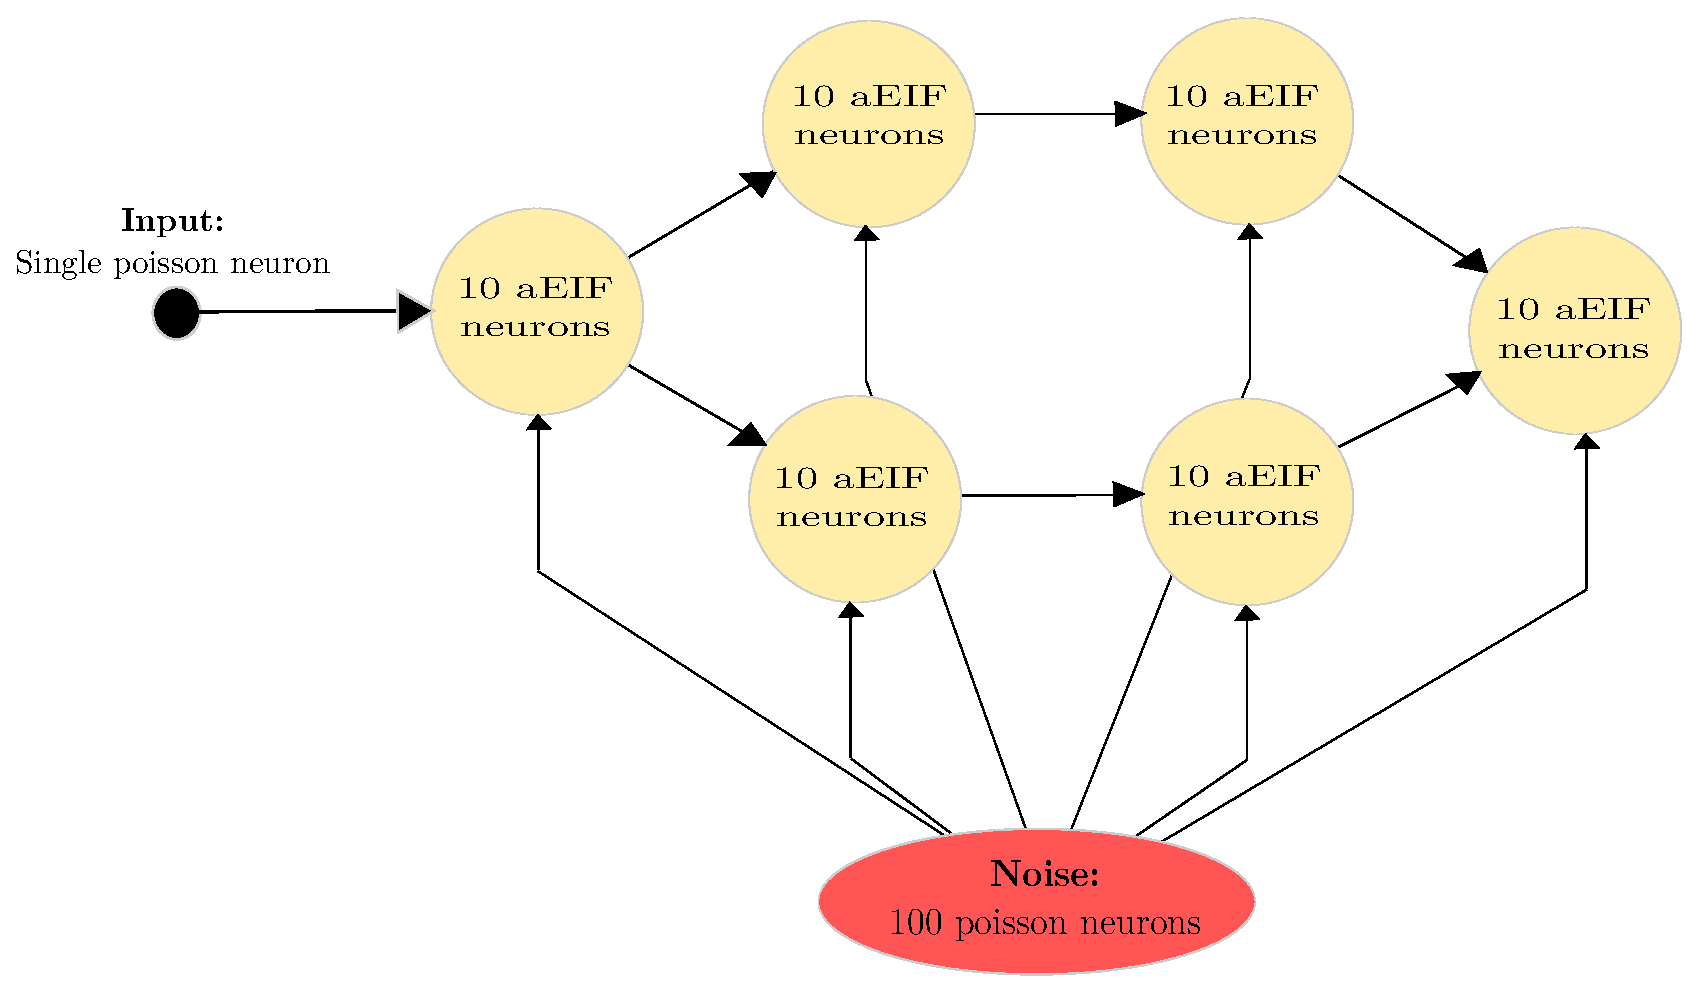
\includegraphics[width=0.9\textwidth]{modelnetwork.eps}
  \bigskip
  \rule{35em}{0.5pt}
  \caption{\label{modelnetwork}The network model which was used to test the effectiveness of the incremental mutual information was based on the schematic shown here.  All simulated neurons in the recurrent layer were aEIF neurons.  The connection probability between two nodes at random was $0.1$, connections along arrows in the diagram occurred with probability $0.8$, and connections from the noise layer to the recurrent layer occurred with probability $0.2$.}
\end{figure}

IMI requires very long data sets to calculate accurately, which are very difficult to record in animals that are awake. Due to the scarcity of  large simultaneous recordings of for long periods of time, the proposed information mapping was instead carried out on a model network.  The network was designed to be small, for ease of calculations, but still had features of note - a divergence and a convergence of groups.  The network was randomly generated based on the schematic in figure \ref{modelnetwork}.  The neuron-model used was the adaptive exponential integrate and fire neuron-model of \citep{BretteGerstner2005a}, as it strikes a good balance between being ease of computation \citep{HopfieldHerz1995a}, and biological accuracy \citep{HodgkinHuxley1952a}.  The network was simulated using the python package Brian \citep{GoodmanBrette2008a}, and each simulation ran for four minutes.  The amplitude of the spikes from the Poisson neurons in the noise layer was varied from 1 mV to 17 mV to investigate how well the IMI dealt with noise.

\begin{figure}[h!]
\centering
\linespread{2}
\begin{tabular}{ll}
{\bf (a)} & {\bf (b)}\\
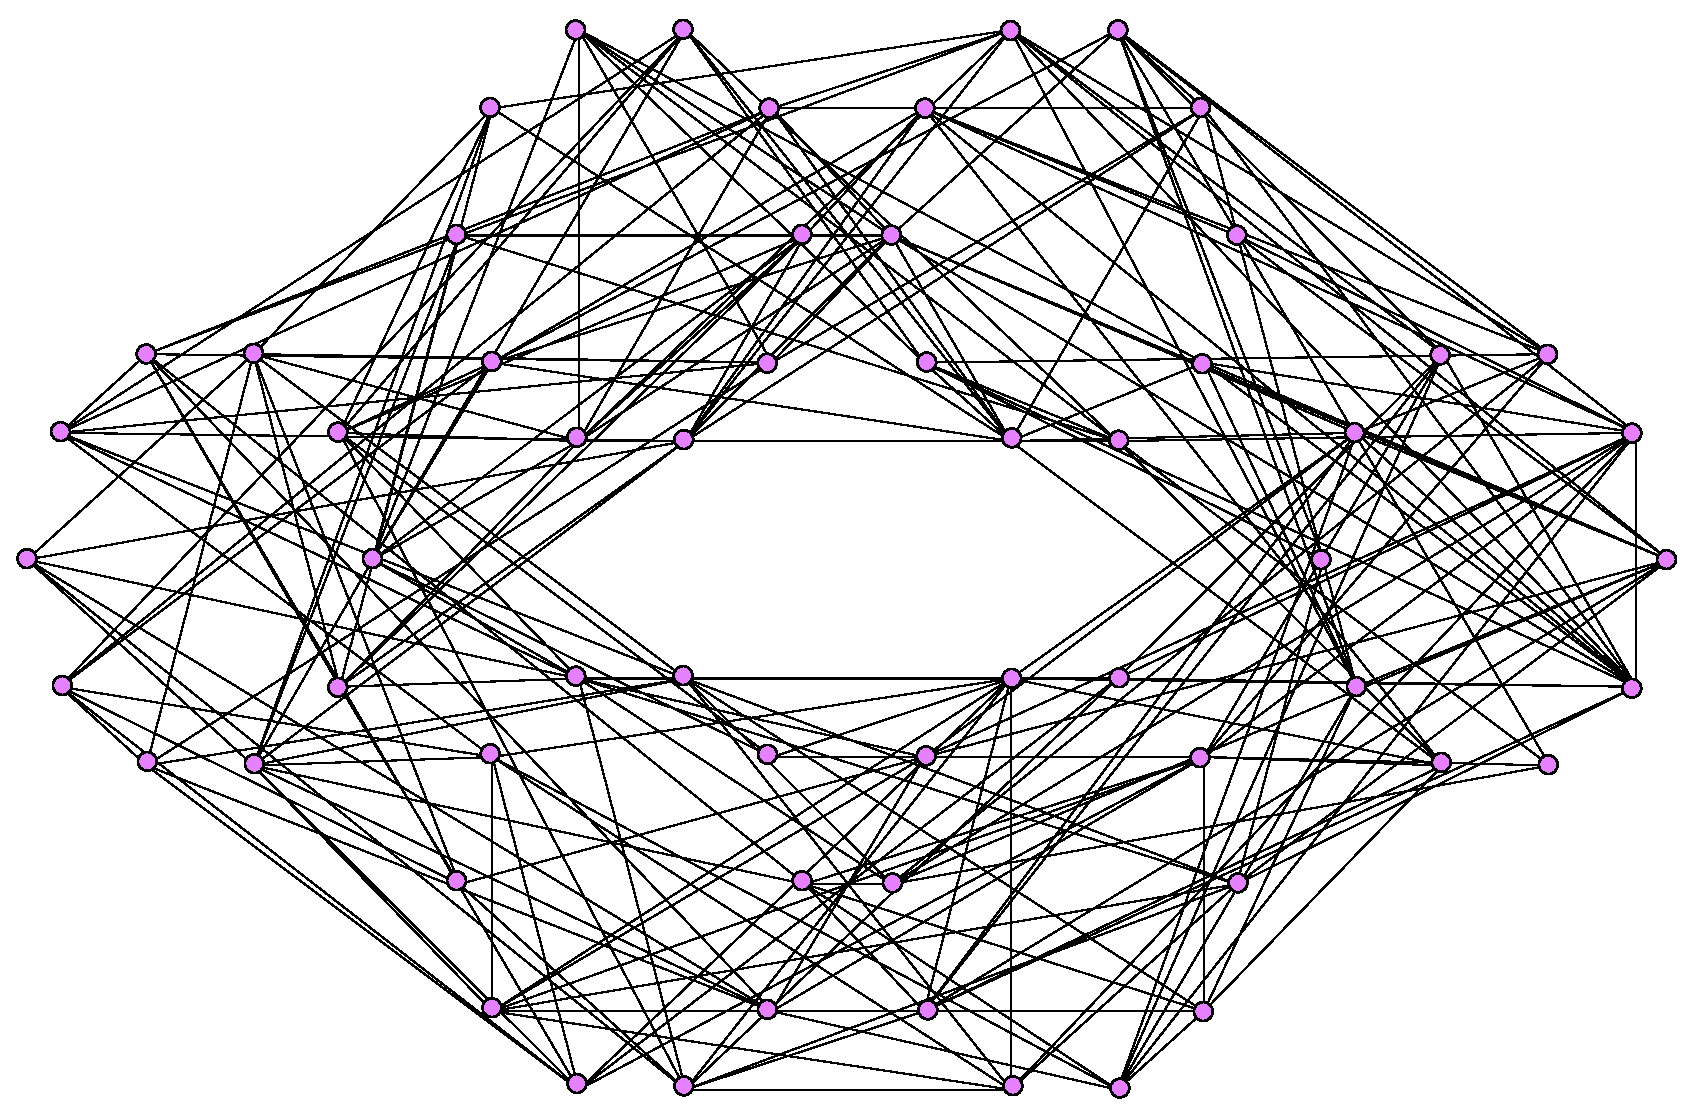
\epsfig{file=directednetnodes.eps,width=0.4\textwidth}
 & \resizebox{0.4\textwidth}{!}{% GNUPLOT: LaTeX picture with Postscript
\begingroup
  \makeatletter
  \providecommand\color[2][]{%
    \GenericError{(gnuplot) \space\space\space\@spaces}{%
      Package color not loaded in conjunction with
      terminal option `colourtext'%
    }{See the gnuplot documentation for explanation.%
    }{Either use 'blacktext' in gnuplot or load the package
      color.sty in LaTeX.}%
    \renewcommand\color[2][]{}%
  }%
  \providecommand\includegraphics[2][]{%
    \GenericError{(gnuplot) \space\space\space\@spaces}{%
      Package graphicx or graphics not loaded%
    }{See the gnuplot documentation for explanation.%
    }{The gnuplot epslatex terminal needs graphicx.sty or graphics.sty.}%
    \renewcommand\includegraphics[2][]{}%
  }%
  \providecommand\rotatebox[2]{#2}%
  \@ifundefined{ifGPcolor}{%
    \newif\ifGPcolor
    \GPcolortrue
  }{}%
  \@ifundefined{ifGPblacktext}{%
    \newif\ifGPblacktext
    \GPblacktexttrue
  }{}%
  % define a \g@addto@macro without @ in the name:
  \let\gplgaddtomacro\g@addto@macro
  % define empty templates for all commands taking text:
  \gdef\gplbacktext{}%
  \gdef\gplfronttext{}%
  \makeatother
  \ifGPblacktext
    % no textcolor at all
    \def\colorrgb#1{}%
    \def\colorgray#1{}%
  \else
    % gray or color?
    \ifGPcolor
      \def\colorrgb#1{\color[rgb]{#1}}%
      \def\colorgray#1{\color[gray]{#1}}%
      \expandafter\def\csname LTw\endcsname{\color{white}}%
      \expandafter\def\csname LTb\endcsname{\color{black}}%
      \expandafter\def\csname LTa\endcsname{\color{black}}%
      \expandafter\def\csname LT0\endcsname{\color[rgb]{1,0,0}}%
      \expandafter\def\csname LT1\endcsname{\color[rgb]{0,1,0}}%
      \expandafter\def\csname LT2\endcsname{\color[rgb]{0,0,1}}%
      \expandafter\def\csname LT3\endcsname{\color[rgb]{1,0,1}}%
      \expandafter\def\csname LT4\endcsname{\color[rgb]{0,1,1}}%
      \expandafter\def\csname LT5\endcsname{\color[rgb]{1,1,0}}%
      \expandafter\def\csname LT6\endcsname{\color[rgb]{0,0,0}}%
      \expandafter\def\csname LT7\endcsname{\color[rgb]{1,0.3,0}}%
      \expandafter\def\csname LT8\endcsname{\color[rgb]{0.5,0.5,0.5}}%
    \else
      % gray
      \def\colorrgb#1{\color{black}}%
      \def\colorgray#1{\color[gray]{#1}}%
      \expandafter\def\csname LTw\endcsname{\color{white}}%
      \expandafter\def\csname LTb\endcsname{\color{black}}%
      \expandafter\def\csname LTa\endcsname{\color{black}}%
      \expandafter\def\csname LT0\endcsname{\color{black}}%
      \expandafter\def\csname LT1\endcsname{\color{black}}%
      \expandafter\def\csname LT2\endcsname{\color{black}}%
      \expandafter\def\csname LT3\endcsname{\color{black}}%
      \expandafter\def\csname LT4\endcsname{\color{black}}%
      \expandafter\def\csname LT5\endcsname{\color{black}}%
      \expandafter\def\csname LT6\endcsname{\color{black}}%
      \expandafter\def\csname LT7\endcsname{\color{black}}%
      \expandafter\def\csname LT8\endcsname{\color{black}}%
    \fi
  \fi
  \setlength{\unitlength}{0.0500bp}%
  \begin{picture}(7200.00,5040.00)%
    \gplgaddtomacro\gplbacktext{%
      \csname LTb\endcsname%
      \put(594,503){\makebox(0,0)[r]{\strut{} 0}}%
      \put(594,1215){\makebox(0,0)[r]{\strut{} 10}}%
      \put(594,1927){\makebox(0,0)[r]{\strut{} 20}}%
      \put(594,2639){\makebox(0,0)[r]{\strut{} 30}}%
      \put(594,3351){\makebox(0,0)[r]{\strut{} 40}}%
      \put(594,4063){\makebox(0,0)[r]{\strut{} 50}}%
      \put(594,4775){\makebox(0,0)[r]{\strut{} 60}}%
      \put(789,220){\makebox(0,0){\strut{} 0}}%
      \put(1623,220){\makebox(0,0){\strut{} 10}}%
      \put(2457,220){\makebox(0,0){\strut{} 20}}%
      \put(3291,220){\makebox(0,0){\strut{} 30}}%
      \put(4124,220){\makebox(0,0){\strut{} 40}}%
      \put(4958,220){\makebox(0,0){\strut{} 50}}%
      \put(5792,220){\makebox(0,0){\strut{} 60}}%
    }%
    \gplgaddtomacro\gplfronttext{%
      \csname LTb\endcsname%
      \put(6362,503){\makebox(0,0)[l]{\strut{} 0}}%
      \put(6362,1037){\makebox(0,0)[l]{\strut{} 0.1}}%
      \put(6362,1571){\makebox(0,0)[l]{\strut{} 0.2}}%
      \put(6362,2105){\makebox(0,0)[l]{\strut{} 0.3}}%
      \put(6362,2639){\makebox(0,0)[l]{\strut{} 0.4}}%
      \put(6362,3173){\makebox(0,0)[l]{\strut{} 0.5}}%
      \put(6362,3706){\makebox(0,0)[l]{\strut{} 0.6}}%
      \put(6362,4241){\makebox(0,0)[l]{\strut{} 0.7}}%
      \put(6362,4774){\makebox(0,0)[l]{\strut{} 0.8}}%
    }%
    \gplbacktext
    \put(0,0){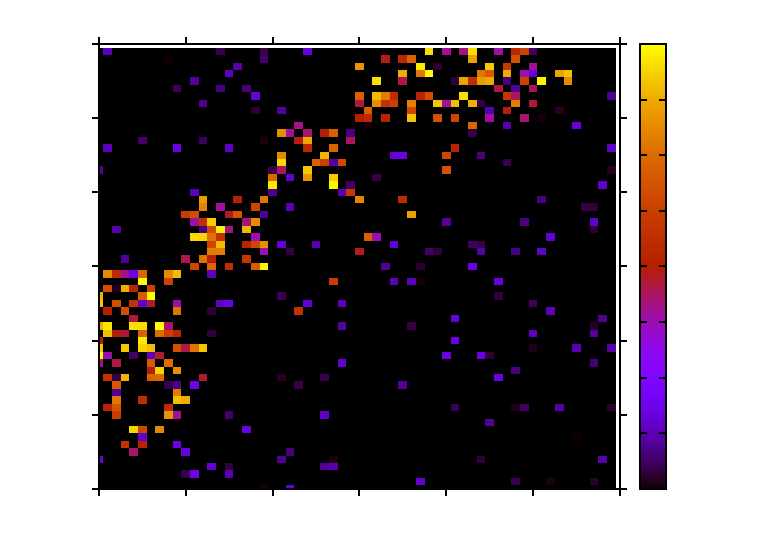
\includegraphics{conn1}}%
    \gplfronttext
  \end{picture}%
\endgroup
}
\end{tabular}
\bigskip
\rule{35em}{0.5pt}
\caption{\label{netwm} {\bf (a)} A typical visualisation of the directed network, very difficult to see what sort of modules exist, despite the layout. {\bf (b) } A heat map of the adjacency matrix of the recurrent layer of aEIF neurons, again there is are very few clusters around the diagonal here, which would indicate a module in the network.}
\end{figure}

The proposed method to map the modules of neurons was to initially calculate the peak IMI between each pair of neurons, and determine the non-diagonal elements of an adjacency matrix of a weighted directed network:
\begin{equation}
A_{ij} = \left\{ \begin{array}{ll} \max_{\delta} \Delta I_{ij}[\delta] & \text{if } \delta>0 \\ 0 & \text{otherwise} \end{array}\right.
\end{equation}

The absolute value of the IMI was quite small, particularly as the noise level increased, but the important information was in the discriminability of the measure.  Therefore, the non-zero IMI values were collected and the median was calculated.  This median, $\tau_I$ was then set as the threshold for the network.  The new adjacency matrix was then calculated as:
\begin{equation}\label{adjmat}
A_{ij, \tau_I} = \left\{ \begin{array}{ll} 1 & \text{if } \max_{\delta} \Delta I_{ij}[\delta] > \tau_I \\ 0 &  \text{otherwise}. \end{array} \right.
\end{equation}

\begin{figure}[htb]
\begin{center}
\begin{tabular}{lll}
{\bf (i)} & {\bf (ii)} & {\bf (iii)} \\
\resizebox{0.3\textwidth}{!}{% GNUPLOT: LaTeX picture with Postscript
\begingroup
  \makeatletter
  \providecommand\color[2][]{%
    \GenericError{(gnuplot) \space\space\space\@spaces}{%
      Package color not loaded in conjunction with
      terminal option `colourtext'%
    }{See the gnuplot documentation for explanation.%
    }{Either use 'blacktext' in gnuplot or load the package
      color.sty in LaTeX.}%
    \renewcommand\color[2][]{}%
  }%
  \providecommand\includegraphics[2][]{%
    \GenericError{(gnuplot) \space\space\space\@spaces}{%
      Package graphicx or graphics not loaded%
    }{See the gnuplot documentation for explanation.%
    }{The gnuplot epslatex terminal needs graphicx.sty or graphics.sty.}%
    \renewcommand\includegraphics[2][]{}%
  }%
  \providecommand\rotatebox[2]{#2}%
  \@ifundefined{ifGPcolor}{%
    \newif\ifGPcolor
    \GPcolortrue
  }{}%
  \@ifundefined{ifGPblacktext}{%
    \newif\ifGPblacktext
    \GPblacktexttrue
  }{}%
  % define a \g@addto@macro without @ in the name:
  \let\gplgaddtomacro\g@addto@macro
  % define empty templates for all commands taking text:
  \gdef\gplbacktext{}%
  \gdef\gplfronttext{}%
  \makeatother
  \ifGPblacktext
    % no textcolor at all
    \def\colorrgb#1{}%
    \def\colorgray#1{}%
  \else
    % gray or color?
    \ifGPcolor
      \def\colorrgb#1{\color[rgb]{#1}}%
      \def\colorgray#1{\color[gray]{#1}}%
      \expandafter\def\csname LTw\endcsname{\color{white}}%
      \expandafter\def\csname LTb\endcsname{\color{black}}%
      \expandafter\def\csname LTa\endcsname{\color{black}}%
      \expandafter\def\csname LT0\endcsname{\color[rgb]{1,0,0}}%
      \expandafter\def\csname LT1\endcsname{\color[rgb]{0,1,0}}%
      \expandafter\def\csname LT2\endcsname{\color[rgb]{0,0,1}}%
      \expandafter\def\csname LT3\endcsname{\color[rgb]{1,0,1}}%
      \expandafter\def\csname LT4\endcsname{\color[rgb]{0,1,1}}%
      \expandafter\def\csname LT5\endcsname{\color[rgb]{1,1,0}}%
      \expandafter\def\csname LT6\endcsname{\color[rgb]{0,0,0}}%
      \expandafter\def\csname LT7\endcsname{\color[rgb]{1,0.3,0}}%
      \expandafter\def\csname LT8\endcsname{\color[rgb]{0.5,0.5,0.5}}%
    \else
      % gray
      \def\colorrgb#1{\color{black}}%
      \def\colorgray#1{\color[gray]{#1}}%
      \expandafter\def\csname LTw\endcsname{\color{white}}%
      \expandafter\def\csname LTb\endcsname{\color{black}}%
      \expandafter\def\csname LTa\endcsname{\color{black}}%
      \expandafter\def\csname LT0\endcsname{\color{black}}%
      \expandafter\def\csname LT1\endcsname{\color{black}}%
      \expandafter\def\csname LT2\endcsname{\color{black}}%
      \expandafter\def\csname LT3\endcsname{\color{black}}%
      \expandafter\def\csname LT4\endcsname{\color{black}}%
      \expandafter\def\csname LT5\endcsname{\color{black}}%
      \expandafter\def\csname LT6\endcsname{\color{black}}%
      \expandafter\def\csname LT7\endcsname{\color{black}}%
      \expandafter\def\csname LT8\endcsname{\color{black}}%
    \fi
  \fi
  \setlength{\unitlength}{0.0500bp}%
  \begin{picture}(7200.00,5040.00)%
    \gplgaddtomacro\gplbacktext{%
      \csname LTb\endcsname%
      \put(594,503){\makebox(0,0)[r]{\strut{} 0}}%
      \put(594,1215){\makebox(0,0)[r]{\strut{} 10}}%
      \put(594,1927){\makebox(0,0)[r]{\strut{} 20}}%
      \put(594,2639){\makebox(0,0)[r]{\strut{} 30}}%
      \put(594,3351){\makebox(0,0)[r]{\strut{} 40}}%
      \put(594,4063){\makebox(0,0)[r]{\strut{} 50}}%
      \put(594,4775){\makebox(0,0)[r]{\strut{} 60}}%
      \put(789,220){\makebox(0,0){\strut{} 0}}%
      \put(1623,220){\makebox(0,0){\strut{} 10}}%
      \put(2457,220){\makebox(0,0){\strut{} 20}}%
      \put(3291,220){\makebox(0,0){\strut{} 30}}%
      \put(4124,220){\makebox(0,0){\strut{} 40}}%
      \put(4958,220){\makebox(0,0){\strut{} 50}}%
      \put(5792,220){\makebox(0,0){\strut{} 60}}%
    }%
    \gplgaddtomacro\gplfronttext{%
      \csname LTb\endcsname%
      \put(6362,503){\makebox(0,0)[l]{\strut{} 0}}%
      \put(6362,1037){\makebox(0,0)[l]{\strut{} 0.1}}%
      \put(6362,1571){\makebox(0,0)[l]{\strut{} 0.2}}%
      \put(6362,2105){\makebox(0,0)[l]{\strut{} 0.3}}%
      \put(6362,2639){\makebox(0,0)[l]{\strut{} 0.4}}%
      \put(6362,3173){\makebox(0,0)[l]{\strut{} 0.5}}%
      \put(6362,3706){\makebox(0,0)[l]{\strut{} 0.6}}%
      \put(6362,4241){\makebox(0,0)[l]{\strut{} 0.7}}%
      \put(6362,4774){\makebox(0,0)[l]{\strut{} 0.8}}%
    }%
    \gplbacktext
    \put(0,0){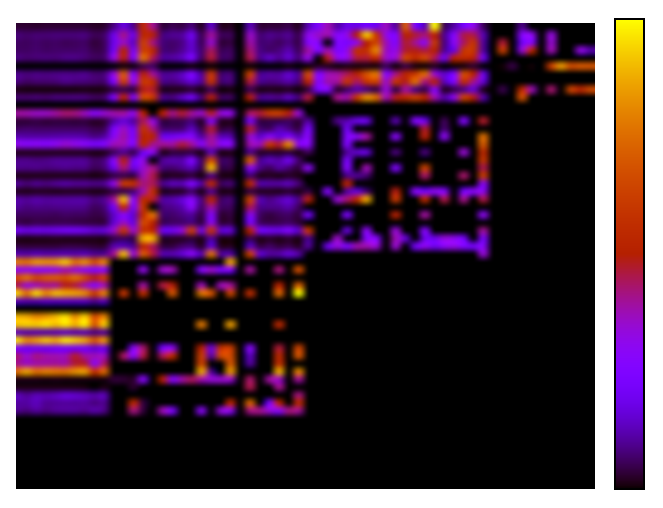
\includegraphics{IMI1}}%
    \gplfronttext
  \end{picture}%
\endgroup
} & \resizebox{0.3\textwidth}{!}{% GNUPLOT: LaTeX picture with Postscript
\begingroup
  \makeatletter
  \providecommand\color[2][]{%
    \GenericError{(gnuplot) \space\space\space\@spaces}{%
      Package color not loaded in conjunction with
      terminal option `colourtext'%
    }{See the gnuplot documentation for explanation.%
    }{Either use 'blacktext' in gnuplot or load the package
      color.sty in LaTeX.}%
    \renewcommand\color[2][]{}%
  }%
  \providecommand\includegraphics[2][]{%
    \GenericError{(gnuplot) \space\space\space\@spaces}{%
      Package graphicx or graphics not loaded%
    }{See the gnuplot documentation for explanation.%
    }{The gnuplot epslatex terminal needs graphicx.sty or graphics.sty.}%
    \renewcommand\includegraphics[2][]{}%
  }%
  \providecommand\rotatebox[2]{#2}%
  \@ifundefined{ifGPcolor}{%
    \newif\ifGPcolor
    \GPcolortrue
  }{}%
  \@ifundefined{ifGPblacktext}{%
    \newif\ifGPblacktext
    \GPblacktexttrue
  }{}%
  % define a \g@addto@macro without @ in the name:
  \let\gplgaddtomacro\g@addto@macro
  % define empty templates for all commands taking text:
  \gdef\gplbacktext{}%
  \gdef\gplfronttext{}%
  \makeatother
  \ifGPblacktext
    % no textcolor at all
    \def\colorrgb#1{}%
    \def\colorgray#1{}%
  \else
    % gray or color?
    \ifGPcolor
      \def\colorrgb#1{\color[rgb]{#1}}%
      \def\colorgray#1{\color[gray]{#1}}%
      \expandafter\def\csname LTw\endcsname{\color{white}}%
      \expandafter\def\csname LTb\endcsname{\color{black}}%
      \expandafter\def\csname LTa\endcsname{\color{black}}%
      \expandafter\def\csname LT0\endcsname{\color[rgb]{1,0,0}}%
      \expandafter\def\csname LT1\endcsname{\color[rgb]{0,1,0}}%
      \expandafter\def\csname LT2\endcsname{\color[rgb]{0,0,1}}%
      \expandafter\def\csname LT3\endcsname{\color[rgb]{1,0,1}}%
      \expandafter\def\csname LT4\endcsname{\color[rgb]{0,1,1}}%
      \expandafter\def\csname LT5\endcsname{\color[rgb]{1,1,0}}%
      \expandafter\def\csname LT6\endcsname{\color[rgb]{0,0,0}}%
      \expandafter\def\csname LT7\endcsname{\color[rgb]{1,0.3,0}}%
      \expandafter\def\csname LT8\endcsname{\color[rgb]{0.5,0.5,0.5}}%
    \else
      % gray
      \def\colorrgb#1{\color{black}}%
      \def\colorgray#1{\color[gray]{#1}}%
      \expandafter\def\csname LTw\endcsname{\color{white}}%
      \expandafter\def\csname LTb\endcsname{\color{black}}%
      \expandafter\def\csname LTa\endcsname{\color{black}}%
      \expandafter\def\csname LT0\endcsname{\color{black}}%
      \expandafter\def\csname LT1\endcsname{\color{black}}%
      \expandafter\def\csname LT2\endcsname{\color{black}}%
      \expandafter\def\csname LT3\endcsname{\color{black}}%
      \expandafter\def\csname LT4\endcsname{\color{black}}%
      \expandafter\def\csname LT5\endcsname{\color{black}}%
      \expandafter\def\csname LT6\endcsname{\color{black}}%
      \expandafter\def\csname LT7\endcsname{\color{black}}%
      \expandafter\def\csname LT8\endcsname{\color{black}}%
    \fi
  \fi
  \setlength{\unitlength}{0.0500bp}%
  \begin{picture}(7200.00,5040.00)%
    \gplgaddtomacro\gplbacktext{%
      \csname LTb\endcsname%
      \put(594,503){\makebox(0,0)[r]{\strut{} 0}}%
      \put(594,1215){\makebox(0,0)[r]{\strut{} 10}}%
      \put(594,1927){\makebox(0,0)[r]{\strut{} 20}}%
      \put(594,2639){\makebox(0,0)[r]{\strut{} 30}}%
      \put(594,3351){\makebox(0,0)[r]{\strut{} 40}}%
      \put(594,4063){\makebox(0,0)[r]{\strut{} 50}}%
      \put(594,4775){\makebox(0,0)[r]{\strut{} 60}}%
      \put(789,220){\makebox(0,0){\strut{} 0}}%
      \put(1623,220){\makebox(0,0){\strut{} 10}}%
      \put(2457,220){\makebox(0,0){\strut{} 20}}%
      \put(3291,220){\makebox(0,0){\strut{} 30}}%
      \put(4124,220){\makebox(0,0){\strut{} 40}}%
      \put(4958,220){\makebox(0,0){\strut{} 50}}%
      \put(5792,220){\makebox(0,0){\strut{} 60}}%
    }%
    \gplgaddtomacro\gplfronttext{%
      \csname LTb\endcsname%
      \put(6362,503){\makebox(0,0)[l]{\strut{} 0}}%
      \put(6362,977){\makebox(0,0)[l]{\strut{} 0.1}}%
      \put(6362,1452){\makebox(0,0)[l]{\strut{} 0.2}}%
      \put(6362,1927){\makebox(0,0)[l]{\strut{} 0.3}}%
      \put(6362,2401){\makebox(0,0)[l]{\strut{} 0.4}}%
      \put(6362,2876){\makebox(0,0)[l]{\strut{} 0.5}}%
      \put(6362,3351){\makebox(0,0)[l]{\strut{} 0.6}}%
      \put(6362,3825){\makebox(0,0)[l]{\strut{} 0.7}}%
      \put(6362,4300){\makebox(0,0)[l]{\strut{} 0.8}}%
      \put(6362,4774){\makebox(0,0)[l]{\strut{} 0.9}}%
    }%
    \gplbacktext
    \put(0,0){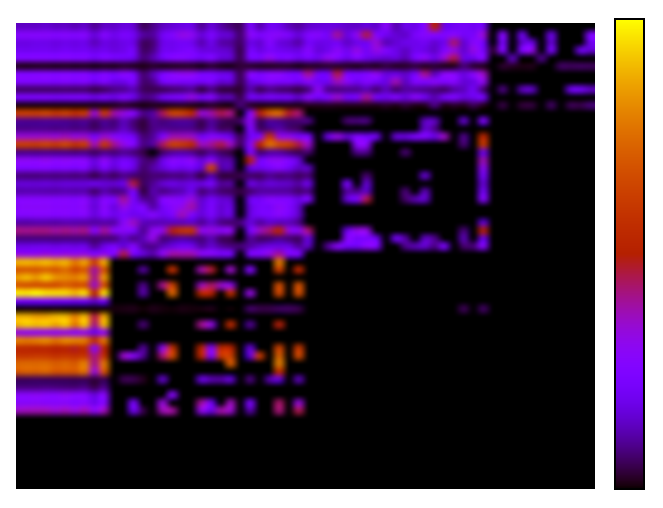
\includegraphics{IMI3}}%
    \gplfronttext
  \end{picture}%
\endgroup
} & \resizebox{0.3\textwidth}{!}{% GNUPLOT: LaTeX picture with Postscript
\begingroup
  \makeatletter
  \providecommand\color[2][]{%
    \GenericError{(gnuplot) \space\space\space\@spaces}{%
      Package color not loaded in conjunction with
      terminal option `colourtext'%
    }{See the gnuplot documentation for explanation.%
    }{Either use 'blacktext' in gnuplot or load the package
      color.sty in LaTeX.}%
    \renewcommand\color[2][]{}%
  }%
  \providecommand\includegraphics[2][]{%
    \GenericError{(gnuplot) \space\space\space\@spaces}{%
      Package graphicx or graphics not loaded%
    }{See the gnuplot documentation for explanation.%
    }{The gnuplot epslatex terminal needs graphicx.sty or graphics.sty.}%
    \renewcommand\includegraphics[2][]{}%
  }%
  \providecommand\rotatebox[2]{#2}%
  \@ifundefined{ifGPcolor}{%
    \newif\ifGPcolor
    \GPcolortrue
  }{}%
  \@ifundefined{ifGPblacktext}{%
    \newif\ifGPblacktext
    \GPblacktexttrue
  }{}%
  % define a \g@addto@macro without @ in the name:
  \let\gplgaddtomacro\g@addto@macro
  % define empty templates for all commands taking text:
  \gdef\gplbacktext{}%
  \gdef\gplfronttext{}%
  \makeatother
  \ifGPblacktext
    % no textcolor at all
    \def\colorrgb#1{}%
    \def\colorgray#1{}%
  \else
    % gray or color?
    \ifGPcolor
      \def\colorrgb#1{\color[rgb]{#1}}%
      \def\colorgray#1{\color[gray]{#1}}%
      \expandafter\def\csname LTw\endcsname{\color{white}}%
      \expandafter\def\csname LTb\endcsname{\color{black}}%
      \expandafter\def\csname LTa\endcsname{\color{black}}%
      \expandafter\def\csname LT0\endcsname{\color[rgb]{1,0,0}}%
      \expandafter\def\csname LT1\endcsname{\color[rgb]{0,1,0}}%
      \expandafter\def\csname LT2\endcsname{\color[rgb]{0,0,1}}%
      \expandafter\def\csname LT3\endcsname{\color[rgb]{1,0,1}}%
      \expandafter\def\csname LT4\endcsname{\color[rgb]{0,1,1}}%
      \expandafter\def\csname LT5\endcsname{\color[rgb]{1,1,0}}%
      \expandafter\def\csname LT6\endcsname{\color[rgb]{0,0,0}}%
      \expandafter\def\csname LT7\endcsname{\color[rgb]{1,0.3,0}}%
      \expandafter\def\csname LT8\endcsname{\color[rgb]{0.5,0.5,0.5}}%
    \else
      % gray
      \def\colorrgb#1{\color{black}}%
      \def\colorgray#1{\color[gray]{#1}}%
      \expandafter\def\csname LTw\endcsname{\color{white}}%
      \expandafter\def\csname LTb\endcsname{\color{black}}%
      \expandafter\def\csname LTa\endcsname{\color{black}}%
      \expandafter\def\csname LT0\endcsname{\color{black}}%
      \expandafter\def\csname LT1\endcsname{\color{black}}%
      \expandafter\def\csname LT2\endcsname{\color{black}}%
      \expandafter\def\csname LT3\endcsname{\color{black}}%
      \expandafter\def\csname LT4\endcsname{\color{black}}%
      \expandafter\def\csname LT5\endcsname{\color{black}}%
      \expandafter\def\csname LT6\endcsname{\color{black}}%
      \expandafter\def\csname LT7\endcsname{\color{black}}%
      \expandafter\def\csname LT8\endcsname{\color{black}}%
    \fi
  \fi
  \setlength{\unitlength}{0.0500bp}%
  \begin{picture}(7200.00,5040.00)%
    \gplgaddtomacro\gplbacktext{%
      \csname LTb\endcsname%
      \put(594,503){\makebox(0,0)[r]{\strut{} 0}}%
      \put(594,1215){\makebox(0,0)[r]{\strut{} 10}}%
      \put(594,1927){\makebox(0,0)[r]{\strut{} 20}}%
      \put(594,2639){\makebox(0,0)[r]{\strut{} 30}}%
      \put(594,3351){\makebox(0,0)[r]{\strut{} 40}}%
      \put(594,4063){\makebox(0,0)[r]{\strut{} 50}}%
      \put(594,4775){\makebox(0,0)[r]{\strut{} 60}}%
      \put(789,220){\makebox(0,0){\strut{} 0}}%
      \put(1623,220){\makebox(0,0){\strut{} 10}}%
      \put(2457,220){\makebox(0,0){\strut{} 20}}%
      \put(3291,220){\makebox(0,0){\strut{} 30}}%
      \put(4124,220){\makebox(0,0){\strut{} 40}}%
      \put(4958,220){\makebox(0,0){\strut{} 50}}%
      \put(5792,220){\makebox(0,0){\strut{} 60}}%
    }%
    \gplgaddtomacro\gplfronttext{%
      \csname LTb\endcsname%
      \put(6362,503){\makebox(0,0)[l]{\strut{} 0}}%
      \put(6362,977){\makebox(0,0)[l]{\strut{} 0.05}}%
      \put(6362,1452){\makebox(0,0)[l]{\strut{} 0.1}}%
      \put(6362,1927){\makebox(0,0)[l]{\strut{} 0.15}}%
      \put(6362,2401){\makebox(0,0)[l]{\strut{} 0.2}}%
      \put(6362,2876){\makebox(0,0)[l]{\strut{} 0.25}}%
      \put(6362,3351){\makebox(0,0)[l]{\strut{} 0.3}}%
      \put(6362,3825){\makebox(0,0)[l]{\strut{} 0.35}}%
      \put(6362,4300){\makebox(0,0)[l]{\strut{} 0.4}}%
      \put(6362,4774){\makebox(0,0)[l]{\strut{} 0.45}}%
    }%
    \gplbacktext
    \put(0,0){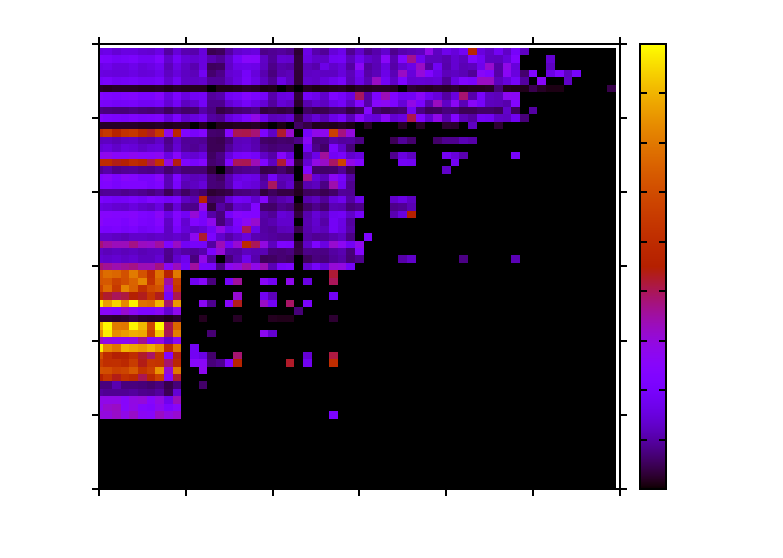
\includegraphics{IMI5}}%
    \gplfronttext
  \end{picture}%
\endgroup
} \\ 
{\bf (iv)} & {\bf (v)} & {\bf (vi)} \\
\resizebox{0.3\textwidth}{!}{% GNUPLOT: LaTeX picture with Postscript
\begingroup
  \makeatletter
  \providecommand\color[2][]{%
    \GenericError{(gnuplot) \space\space\space\@spaces}{%
      Package color not loaded in conjunction with
      terminal option `colourtext'%
    }{See the gnuplot documentation for explanation.%
    }{Either use 'blacktext' in gnuplot or load the package
      color.sty in LaTeX.}%
    \renewcommand\color[2][]{}%
  }%
  \providecommand\includegraphics[2][]{%
    \GenericError{(gnuplot) \space\space\space\@spaces}{%
      Package graphicx or graphics not loaded%
    }{See the gnuplot documentation for explanation.%
    }{The gnuplot epslatex terminal needs graphicx.sty or graphics.sty.}%
    \renewcommand\includegraphics[2][]{}%
  }%
  \providecommand\rotatebox[2]{#2}%
  \@ifundefined{ifGPcolor}{%
    \newif\ifGPcolor
    \GPcolortrue
  }{}%
  \@ifundefined{ifGPblacktext}{%
    \newif\ifGPblacktext
    \GPblacktexttrue
  }{}%
  % define a \g@addto@macro without @ in the name:
  \let\gplgaddtomacro\g@addto@macro
  % define empty templates for all commands taking text:
  \gdef\gplbacktext{}%
  \gdef\gplfronttext{}%
  \makeatother
  \ifGPblacktext
    % no textcolor at all
    \def\colorrgb#1{}%
    \def\colorgray#1{}%
  \else
    % gray or color?
    \ifGPcolor
      \def\colorrgb#1{\color[rgb]{#1}}%
      \def\colorgray#1{\color[gray]{#1}}%
      \expandafter\def\csname LTw\endcsname{\color{white}}%
      \expandafter\def\csname LTb\endcsname{\color{black}}%
      \expandafter\def\csname LTa\endcsname{\color{black}}%
      \expandafter\def\csname LT0\endcsname{\color[rgb]{1,0,0}}%
      \expandafter\def\csname LT1\endcsname{\color[rgb]{0,1,0}}%
      \expandafter\def\csname LT2\endcsname{\color[rgb]{0,0,1}}%
      \expandafter\def\csname LT3\endcsname{\color[rgb]{1,0,1}}%
      \expandafter\def\csname LT4\endcsname{\color[rgb]{0,1,1}}%
      \expandafter\def\csname LT5\endcsname{\color[rgb]{1,1,0}}%
      \expandafter\def\csname LT6\endcsname{\color[rgb]{0,0,0}}%
      \expandafter\def\csname LT7\endcsname{\color[rgb]{1,0.3,0}}%
      \expandafter\def\csname LT8\endcsname{\color[rgb]{0.5,0.5,0.5}}%
    \else
      % gray
      \def\colorrgb#1{\color{black}}%
      \def\colorgray#1{\color[gray]{#1}}%
      \expandafter\def\csname LTw\endcsname{\color{white}}%
      \expandafter\def\csname LTb\endcsname{\color{black}}%
      \expandafter\def\csname LTa\endcsname{\color{black}}%
      \expandafter\def\csname LT0\endcsname{\color{black}}%
      \expandafter\def\csname LT1\endcsname{\color{black}}%
      \expandafter\def\csname LT2\endcsname{\color{black}}%
      \expandafter\def\csname LT3\endcsname{\color{black}}%
      \expandafter\def\csname LT4\endcsname{\color{black}}%
      \expandafter\def\csname LT5\endcsname{\color{black}}%
      \expandafter\def\csname LT6\endcsname{\color{black}}%
      \expandafter\def\csname LT7\endcsname{\color{black}}%
      \expandafter\def\csname LT8\endcsname{\color{black}}%
    \fi
  \fi
  \setlength{\unitlength}{0.0500bp}%
  \begin{picture}(7200.00,5040.00)%
    \gplgaddtomacro\gplbacktext{%
      \csname LTb\endcsname%
      \put(594,503){\makebox(0,0)[r]{\strut{} 0}}%
      \put(594,1215){\makebox(0,0)[r]{\strut{} 10}}%
      \put(594,1927){\makebox(0,0)[r]{\strut{} 20}}%
      \put(594,2639){\makebox(0,0)[r]{\strut{} 30}}%
      \put(594,3351){\makebox(0,0)[r]{\strut{} 40}}%
      \put(594,4063){\makebox(0,0)[r]{\strut{} 50}}%
      \put(594,4775){\makebox(0,0)[r]{\strut{} 60}}%
      \put(789,220){\makebox(0,0){\strut{} 0}}%
      \put(1623,220){\makebox(0,0){\strut{} 10}}%
      \put(2457,220){\makebox(0,0){\strut{} 20}}%
      \put(3291,220){\makebox(0,0){\strut{} 30}}%
      \put(4124,220){\makebox(0,0){\strut{} 40}}%
      \put(4958,220){\makebox(0,0){\strut{} 50}}%
      \put(5792,220){\makebox(0,0){\strut{} 60}}%
    }%
    \gplgaddtomacro\gplfronttext{%
      \csname LTb\endcsname%
      \put(6362,503){\makebox(0,0)[l]{\strut{} 0}}%
      \put(6362,1215){\makebox(0,0)[l]{\strut{} 0.05}}%
      \put(6362,1927){\makebox(0,0)[l]{\strut{} 0.1}}%
      \put(6362,2639){\makebox(0,0)[l]{\strut{} 0.15}}%
      \put(6362,3351){\makebox(0,0)[l]{\strut{} 0.2}}%
      \put(6362,4062){\makebox(0,0)[l]{\strut{} 0.25}}%
      \put(6362,4774){\makebox(0,0)[l]{\strut{} 0.3}}%
    }%
    \gplbacktext
    \put(0,0){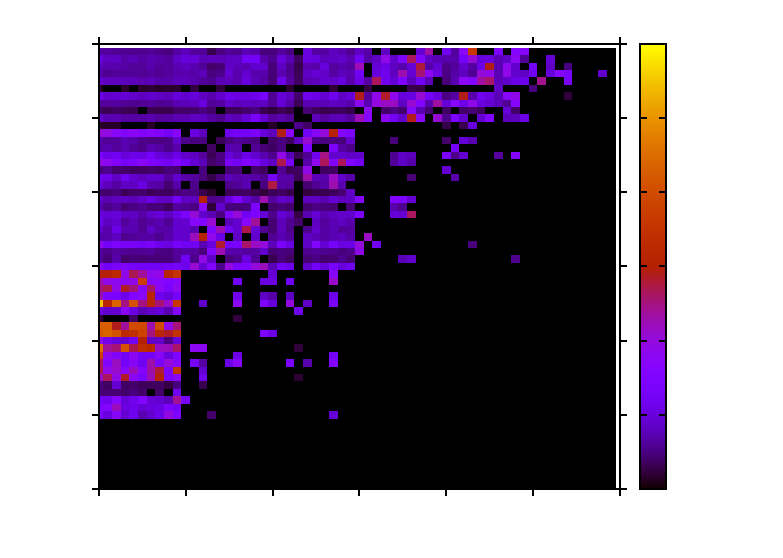
\includegraphics{IMI7}}%
    \gplfronttext
  \end{picture}%
\endgroup
} & \resizebox{0.3\textwidth}{!}{% GNUPLOT: LaTeX picture with Postscript
\begingroup
  \makeatletter
  \providecommand\color[2][]{%
    \GenericError{(gnuplot) \space\space\space\@spaces}{%
      Package color not loaded in conjunction with
      terminal option `colourtext'%
    }{See the gnuplot documentation for explanation.%
    }{Either use 'blacktext' in gnuplot or load the package
      color.sty in LaTeX.}%
    \renewcommand\color[2][]{}%
  }%
  \providecommand\includegraphics[2][]{%
    \GenericError{(gnuplot) \space\space\space\@spaces}{%
      Package graphicx or graphics not loaded%
    }{See the gnuplot documentation for explanation.%
    }{The gnuplot epslatex terminal needs graphicx.sty or graphics.sty.}%
    \renewcommand\includegraphics[2][]{}%
  }%
  \providecommand\rotatebox[2]{#2}%
  \@ifundefined{ifGPcolor}{%
    \newif\ifGPcolor
    \GPcolortrue
  }{}%
  \@ifundefined{ifGPblacktext}{%
    \newif\ifGPblacktext
    \GPblacktexttrue
  }{}%
  % define a \g@addto@macro without @ in the name:
  \let\gplgaddtomacro\g@addto@macro
  % define empty templates for all commands taking text:
  \gdef\gplbacktext{}%
  \gdef\gplfronttext{}%
  \makeatother
  \ifGPblacktext
    % no textcolor at all
    \def\colorrgb#1{}%
    \def\colorgray#1{}%
  \else
    % gray or color?
    \ifGPcolor
      \def\colorrgb#1{\color[rgb]{#1}}%
      \def\colorgray#1{\color[gray]{#1}}%
      \expandafter\def\csname LTw\endcsname{\color{white}}%
      \expandafter\def\csname LTb\endcsname{\color{black}}%
      \expandafter\def\csname LTa\endcsname{\color{black}}%
      \expandafter\def\csname LT0\endcsname{\color[rgb]{1,0,0}}%
      \expandafter\def\csname LT1\endcsname{\color[rgb]{0,1,0}}%
      \expandafter\def\csname LT2\endcsname{\color[rgb]{0,0,1}}%
      \expandafter\def\csname LT3\endcsname{\color[rgb]{1,0,1}}%
      \expandafter\def\csname LT4\endcsname{\color[rgb]{0,1,1}}%
      \expandafter\def\csname LT5\endcsname{\color[rgb]{1,1,0}}%
      \expandafter\def\csname LT6\endcsname{\color[rgb]{0,0,0}}%
      \expandafter\def\csname LT7\endcsname{\color[rgb]{1,0.3,0}}%
      \expandafter\def\csname LT8\endcsname{\color[rgb]{0.5,0.5,0.5}}%
    \else
      % gray
      \def\colorrgb#1{\color{black}}%
      \def\colorgray#1{\color[gray]{#1}}%
      \expandafter\def\csname LTw\endcsname{\color{white}}%
      \expandafter\def\csname LTb\endcsname{\color{black}}%
      \expandafter\def\csname LTa\endcsname{\color{black}}%
      \expandafter\def\csname LT0\endcsname{\color{black}}%
      \expandafter\def\csname LT1\endcsname{\color{black}}%
      \expandafter\def\csname LT2\endcsname{\color{black}}%
      \expandafter\def\csname LT3\endcsname{\color{black}}%
      \expandafter\def\csname LT4\endcsname{\color{black}}%
      \expandafter\def\csname LT5\endcsname{\color{black}}%
      \expandafter\def\csname LT6\endcsname{\color{black}}%
      \expandafter\def\csname LT7\endcsname{\color{black}}%
      \expandafter\def\csname LT8\endcsname{\color{black}}%
    \fi
  \fi
  \setlength{\unitlength}{0.0500bp}%
  \begin{picture}(7200.00,5040.00)%
    \gplgaddtomacro\gplbacktext{%
      \csname LTb\endcsname%
      \put(594,503){\makebox(0,0)[r]{\strut{} 0}}%
      \put(594,1215){\makebox(0,0)[r]{\strut{} 10}}%
      \put(594,1927){\makebox(0,0)[r]{\strut{} 20}}%
      \put(594,2639){\makebox(0,0)[r]{\strut{} 30}}%
      \put(594,3351){\makebox(0,0)[r]{\strut{} 40}}%
      \put(594,4063){\makebox(0,0)[r]{\strut{} 50}}%
      \put(594,4775){\makebox(0,0)[r]{\strut{} 60}}%
      \put(789,220){\makebox(0,0){\strut{} 0}}%
      \put(1623,220){\makebox(0,0){\strut{} 10}}%
      \put(2457,220){\makebox(0,0){\strut{} 20}}%
      \put(3291,220){\makebox(0,0){\strut{} 30}}%
      \put(4124,220){\makebox(0,0){\strut{} 40}}%
      \put(4958,220){\makebox(0,0){\strut{} 50}}%
      \put(5792,220){\makebox(0,0){\strut{} 60}}%
    }%
    \gplgaddtomacro\gplfronttext{%
      \csname LTb\endcsname%
      \put(6362,503){\makebox(0,0)[l]{\strut{} 0}}%
      \put(6362,930){\makebox(0,0)[l]{\strut{} 0.02}}%
      \put(6362,1357){\makebox(0,0)[l]{\strut{} 0.04}}%
      \put(6362,1784){\makebox(0,0)[l]{\strut{} 0.06}}%
      \put(6362,2211){\makebox(0,0)[l]{\strut{} 0.08}}%
      \put(6362,2639){\makebox(0,0)[l]{\strut{} 0.1}}%
      \put(6362,3066){\makebox(0,0)[l]{\strut{} 0.12}}%
      \put(6362,3493){\makebox(0,0)[l]{\strut{} 0.14}}%
      \put(6362,3920){\makebox(0,0)[l]{\strut{} 0.16}}%
      \put(6362,4347){\makebox(0,0)[l]{\strut{} 0.18}}%
      \put(6362,4775){\makebox(0,0)[l]{\strut{} 0.2}}%
    }%
    \gplbacktext
    \put(0,0){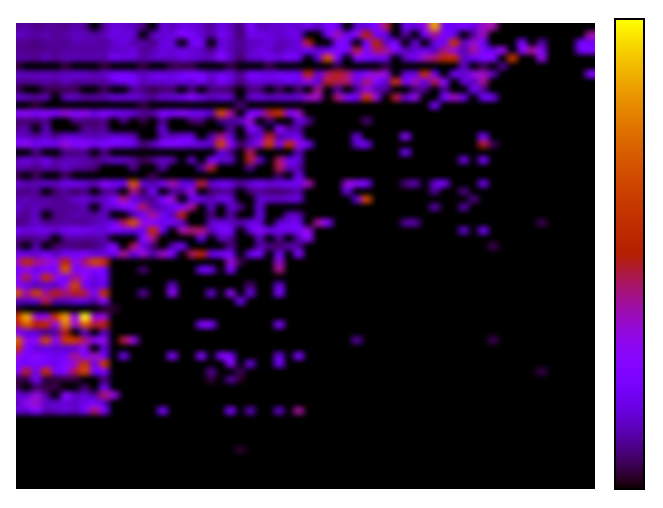
\includegraphics{IMI9}}%
    \gplfronttext
  \end{picture}%
\endgroup
} & \resizebox{0.3\textwidth}{!}{% GNUPLOT: LaTeX picture with Postscript
\begingroup
  \makeatletter
  \providecommand\color[2][]{%
    \GenericError{(gnuplot) \space\space\space\@spaces}{%
      Package color not loaded in conjunction with
      terminal option `colourtext'%
    }{See the gnuplot documentation for explanation.%
    }{Either use 'blacktext' in gnuplot or load the package
      color.sty in LaTeX.}%
    \renewcommand\color[2][]{}%
  }%
  \providecommand\includegraphics[2][]{%
    \GenericError{(gnuplot) \space\space\space\@spaces}{%
      Package graphicx or graphics not loaded%
    }{See the gnuplot documentation for explanation.%
    }{The gnuplot epslatex terminal needs graphicx.sty or graphics.sty.}%
    \renewcommand\includegraphics[2][]{}%
  }%
  \providecommand\rotatebox[2]{#2}%
  \@ifundefined{ifGPcolor}{%
    \newif\ifGPcolor
    \GPcolortrue
  }{}%
  \@ifundefined{ifGPblacktext}{%
    \newif\ifGPblacktext
    \GPblacktexttrue
  }{}%
  % define a \g@addto@macro without @ in the name:
  \let\gplgaddtomacro\g@addto@macro
  % define empty templates for all commands taking text:
  \gdef\gplbacktext{}%
  \gdef\gplfronttext{}%
  \makeatother
  \ifGPblacktext
    % no textcolor at all
    \def\colorrgb#1{}%
    \def\colorgray#1{}%
  \else
    % gray or color?
    \ifGPcolor
      \def\colorrgb#1{\color[rgb]{#1}}%
      \def\colorgray#1{\color[gray]{#1}}%
      \expandafter\def\csname LTw\endcsname{\color{white}}%
      \expandafter\def\csname LTb\endcsname{\color{black}}%
      \expandafter\def\csname LTa\endcsname{\color{black}}%
      \expandafter\def\csname LT0\endcsname{\color[rgb]{1,0,0}}%
      \expandafter\def\csname LT1\endcsname{\color[rgb]{0,1,0}}%
      \expandafter\def\csname LT2\endcsname{\color[rgb]{0,0,1}}%
      \expandafter\def\csname LT3\endcsname{\color[rgb]{1,0,1}}%
      \expandafter\def\csname LT4\endcsname{\color[rgb]{0,1,1}}%
      \expandafter\def\csname LT5\endcsname{\color[rgb]{1,1,0}}%
      \expandafter\def\csname LT6\endcsname{\color[rgb]{0,0,0}}%
      \expandafter\def\csname LT7\endcsname{\color[rgb]{1,0.3,0}}%
      \expandafter\def\csname LT8\endcsname{\color[rgb]{0.5,0.5,0.5}}%
    \else
      % gray
      \def\colorrgb#1{\color{black}}%
      \def\colorgray#1{\color[gray]{#1}}%
      \expandafter\def\csname LTw\endcsname{\color{white}}%
      \expandafter\def\csname LTb\endcsname{\color{black}}%
      \expandafter\def\csname LTa\endcsname{\color{black}}%
      \expandafter\def\csname LT0\endcsname{\color{black}}%
      \expandafter\def\csname LT1\endcsname{\color{black}}%
      \expandafter\def\csname LT2\endcsname{\color{black}}%
      \expandafter\def\csname LT3\endcsname{\color{black}}%
      \expandafter\def\csname LT4\endcsname{\color{black}}%
      \expandafter\def\csname LT5\endcsname{\color{black}}%
      \expandafter\def\csname LT6\endcsname{\color{black}}%
      \expandafter\def\csname LT7\endcsname{\color{black}}%
      \expandafter\def\csname LT8\endcsname{\color{black}}%
    \fi
  \fi
  \setlength{\unitlength}{0.0500bp}%
  \begin{picture}(7200.00,5040.00)%
    \gplgaddtomacro\gplbacktext{%
      \csname LTb\endcsname%
      \put(594,503){\makebox(0,0)[r]{\strut{} 0}}%
      \put(594,1215){\makebox(0,0)[r]{\strut{} 10}}%
      \put(594,1927){\makebox(0,0)[r]{\strut{} 20}}%
      \put(594,2639){\makebox(0,0)[r]{\strut{} 30}}%
      \put(594,3351){\makebox(0,0)[r]{\strut{} 40}}%
      \put(594,4063){\makebox(0,0)[r]{\strut{} 50}}%
      \put(594,4775){\makebox(0,0)[r]{\strut{} 60}}%
      \put(789,220){\makebox(0,0){\strut{} 0}}%
      \put(1623,220){\makebox(0,0){\strut{} 10}}%
      \put(2457,220){\makebox(0,0){\strut{} 20}}%
      \put(3291,220){\makebox(0,0){\strut{} 30}}%
      \put(4124,220){\makebox(0,0){\strut{} 40}}%
      \put(4958,220){\makebox(0,0){\strut{} 50}}%
      \put(5792,220){\makebox(0,0){\strut{} 60}}%
    }%
    \gplgaddtomacro\gplfronttext{%
      \csname LTb\endcsname%
      \put(6362,503){\makebox(0,0)[l]{\strut{} 0}}%
      \put(6362,1113){\makebox(0,0)[l]{\strut{} 0.02}}%
      \put(6362,1723){\makebox(0,0)[l]{\strut{} 0.04}}%
      \put(6362,2333){\makebox(0,0)[l]{\strut{} 0.06}}%
      \put(6362,2944){\makebox(0,0)[l]{\strut{} 0.08}}%
      \put(6362,3554){\makebox(0,0)[l]{\strut{} 0.1}}%
      \put(6362,4164){\makebox(0,0)[l]{\strut{} 0.12}}%
      \put(6362,4775){\makebox(0,0)[l]{\strut{} 0.14}}%
    }%
    \gplbacktext
    \put(0,0){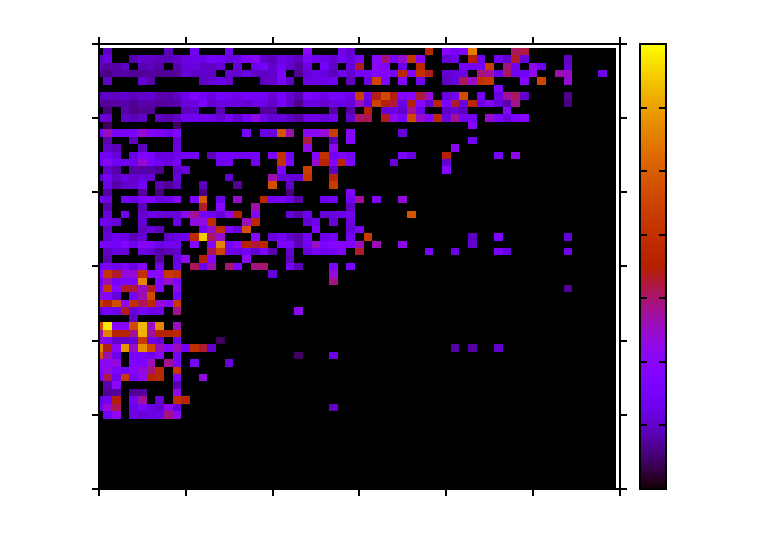
\includegraphics{IMI11}}%
    \gplfronttext
  \end{picture}%
\endgroup
} \\ 
{\bf (vii)} & {\bf (viii)} & {\bf (ix)} \\
\resizebox{0.3\textwidth}{!}{% GNUPLOT: LaTeX picture with Postscript
\begingroup
  \makeatletter
  \providecommand\color[2][]{%
    \GenericError{(gnuplot) \space\space\space\@spaces}{%
      Package color not loaded in conjunction with
      terminal option `colourtext'%
    }{See the gnuplot documentation for explanation.%
    }{Either use 'blacktext' in gnuplot or load the package
      color.sty in LaTeX.}%
    \renewcommand\color[2][]{}%
  }%
  \providecommand\includegraphics[2][]{%
    \GenericError{(gnuplot) \space\space\space\@spaces}{%
      Package graphicx or graphics not loaded%
    }{See the gnuplot documentation for explanation.%
    }{The gnuplot epslatex terminal needs graphicx.sty or graphics.sty.}%
    \renewcommand\includegraphics[2][]{}%
  }%
  \providecommand\rotatebox[2]{#2}%
  \@ifundefined{ifGPcolor}{%
    \newif\ifGPcolor
    \GPcolortrue
  }{}%
  \@ifundefined{ifGPblacktext}{%
    \newif\ifGPblacktext
    \GPblacktexttrue
  }{}%
  % define a \g@addto@macro without @ in the name:
  \let\gplgaddtomacro\g@addto@macro
  % define empty templates for all commands taking text:
  \gdef\gplbacktext{}%
  \gdef\gplfronttext{}%
  \makeatother
  \ifGPblacktext
    % no textcolor at all
    \def\colorrgb#1{}%
    \def\colorgray#1{}%
  \else
    % gray or color?
    \ifGPcolor
      \def\colorrgb#1{\color[rgb]{#1}}%
      \def\colorgray#1{\color[gray]{#1}}%
      \expandafter\def\csname LTw\endcsname{\color{white}}%
      \expandafter\def\csname LTb\endcsname{\color{black}}%
      \expandafter\def\csname LTa\endcsname{\color{black}}%
      \expandafter\def\csname LT0\endcsname{\color[rgb]{1,0,0}}%
      \expandafter\def\csname LT1\endcsname{\color[rgb]{0,1,0}}%
      \expandafter\def\csname LT2\endcsname{\color[rgb]{0,0,1}}%
      \expandafter\def\csname LT3\endcsname{\color[rgb]{1,0,1}}%
      \expandafter\def\csname LT4\endcsname{\color[rgb]{0,1,1}}%
      \expandafter\def\csname LT5\endcsname{\color[rgb]{1,1,0}}%
      \expandafter\def\csname LT6\endcsname{\color[rgb]{0,0,0}}%
      \expandafter\def\csname LT7\endcsname{\color[rgb]{1,0.3,0}}%
      \expandafter\def\csname LT8\endcsname{\color[rgb]{0.5,0.5,0.5}}%
    \else
      % gray
      \def\colorrgb#1{\color{black}}%
      \def\colorgray#1{\color[gray]{#1}}%
      \expandafter\def\csname LTw\endcsname{\color{white}}%
      \expandafter\def\csname LTb\endcsname{\color{black}}%
      \expandafter\def\csname LTa\endcsname{\color{black}}%
      \expandafter\def\csname LT0\endcsname{\color{black}}%
      \expandafter\def\csname LT1\endcsname{\color{black}}%
      \expandafter\def\csname LT2\endcsname{\color{black}}%
      \expandafter\def\csname LT3\endcsname{\color{black}}%
      \expandafter\def\csname LT4\endcsname{\color{black}}%
      \expandafter\def\csname LT5\endcsname{\color{black}}%
      \expandafter\def\csname LT6\endcsname{\color{black}}%
      \expandafter\def\csname LT7\endcsname{\color{black}}%
      \expandafter\def\csname LT8\endcsname{\color{black}}%
    \fi
  \fi
  \setlength{\unitlength}{0.0500bp}%
  \begin{picture}(7200.00,5040.00)%
    \gplgaddtomacro\gplbacktext{%
      \csname LTb\endcsname%
      \put(594,503){\makebox(0,0)[r]{\strut{} 0}}%
      \put(594,1215){\makebox(0,0)[r]{\strut{} 10}}%
      \put(594,1927){\makebox(0,0)[r]{\strut{} 20}}%
      \put(594,2639){\makebox(0,0)[r]{\strut{} 30}}%
      \put(594,3351){\makebox(0,0)[r]{\strut{} 40}}%
      \put(594,4063){\makebox(0,0)[r]{\strut{} 50}}%
      \put(594,4775){\makebox(0,0)[r]{\strut{} 60}}%
      \put(789,220){\makebox(0,0){\strut{} 0}}%
      \put(1623,220){\makebox(0,0){\strut{} 10}}%
      \put(2457,220){\makebox(0,0){\strut{} 20}}%
      \put(3291,220){\makebox(0,0){\strut{} 30}}%
      \put(4124,220){\makebox(0,0){\strut{} 40}}%
      \put(4958,220){\makebox(0,0){\strut{} 50}}%
      \put(5792,220){\makebox(0,0){\strut{} 60}}%
    }%
    \gplgaddtomacro\gplfronttext{%
      \csname LTb\endcsname%
      \put(6362,503){\makebox(0,0)[l]{\strut{} 0}}%
      \put(6362,1215){\makebox(0,0)[l]{\strut{} 0.02}}%
      \put(6362,1927){\makebox(0,0)[l]{\strut{} 0.04}}%
      \put(6362,2639){\makebox(0,0)[l]{\strut{} 0.06}}%
      \put(6362,3351){\makebox(0,0)[l]{\strut{} 0.08}}%
      \put(6362,4063){\makebox(0,0)[l]{\strut{} 0.1}}%
      \put(6362,4775){\makebox(0,0)[l]{\strut{} 0.12}}%
    }%
    \gplbacktext
    \put(0,0){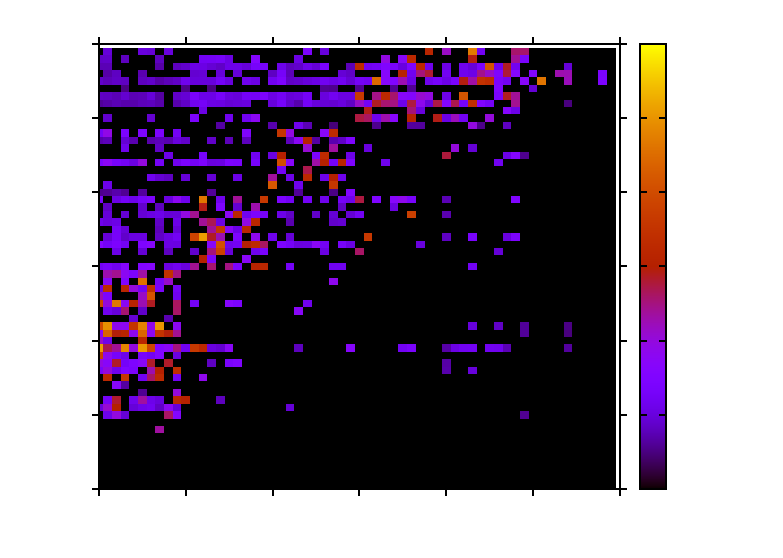
\includegraphics{IMI13}}%
    \gplfronttext
  \end{picture}%
\endgroup
} & \resizebox{0.3\textwidth}{!}{% GNUPLOT: LaTeX picture with Postscript
\begingroup
  \makeatletter
  \providecommand\color[2][]{%
    \GenericError{(gnuplot) \space\space\space\@spaces}{%
      Package color not loaded in conjunction with
      terminal option `colourtext'%
    }{See the gnuplot documentation for explanation.%
    }{Either use 'blacktext' in gnuplot or load the package
      color.sty in LaTeX.}%
    \renewcommand\color[2][]{}%
  }%
  \providecommand\includegraphics[2][]{%
    \GenericError{(gnuplot) \space\space\space\@spaces}{%
      Package graphicx or graphics not loaded%
    }{See the gnuplot documentation for explanation.%
    }{The gnuplot epslatex terminal needs graphicx.sty or graphics.sty.}%
    \renewcommand\includegraphics[2][]{}%
  }%
  \providecommand\rotatebox[2]{#2}%
  \@ifundefined{ifGPcolor}{%
    \newif\ifGPcolor
    \GPcolortrue
  }{}%
  \@ifundefined{ifGPblacktext}{%
    \newif\ifGPblacktext
    \GPblacktexttrue
  }{}%
  % define a \g@addto@macro without @ in the name:
  \let\gplgaddtomacro\g@addto@macro
  % define empty templates for all commands taking text:
  \gdef\gplbacktext{}%
  \gdef\gplfronttext{}%
  \makeatother
  \ifGPblacktext
    % no textcolor at all
    \def\colorrgb#1{}%
    \def\colorgray#1{}%
  \else
    % gray or color?
    \ifGPcolor
      \def\colorrgb#1{\color[rgb]{#1}}%
      \def\colorgray#1{\color[gray]{#1}}%
      \expandafter\def\csname LTw\endcsname{\color{white}}%
      \expandafter\def\csname LTb\endcsname{\color{black}}%
      \expandafter\def\csname LTa\endcsname{\color{black}}%
      \expandafter\def\csname LT0\endcsname{\color[rgb]{1,0,0}}%
      \expandafter\def\csname LT1\endcsname{\color[rgb]{0,1,0}}%
      \expandafter\def\csname LT2\endcsname{\color[rgb]{0,0,1}}%
      \expandafter\def\csname LT3\endcsname{\color[rgb]{1,0,1}}%
      \expandafter\def\csname LT4\endcsname{\color[rgb]{0,1,1}}%
      \expandafter\def\csname LT5\endcsname{\color[rgb]{1,1,0}}%
      \expandafter\def\csname LT6\endcsname{\color[rgb]{0,0,0}}%
      \expandafter\def\csname LT7\endcsname{\color[rgb]{1,0.3,0}}%
      \expandafter\def\csname LT8\endcsname{\color[rgb]{0.5,0.5,0.5}}%
    \else
      % gray
      \def\colorrgb#1{\color{black}}%
      \def\colorgray#1{\color[gray]{#1}}%
      \expandafter\def\csname LTw\endcsname{\color{white}}%
      \expandafter\def\csname LTb\endcsname{\color{black}}%
      \expandafter\def\csname LTa\endcsname{\color{black}}%
      \expandafter\def\csname LT0\endcsname{\color{black}}%
      \expandafter\def\csname LT1\endcsname{\color{black}}%
      \expandafter\def\csname LT2\endcsname{\color{black}}%
      \expandafter\def\csname LT3\endcsname{\color{black}}%
      \expandafter\def\csname LT4\endcsname{\color{black}}%
      \expandafter\def\csname LT5\endcsname{\color{black}}%
      \expandafter\def\csname LT6\endcsname{\color{black}}%
      \expandafter\def\csname LT7\endcsname{\color{black}}%
      \expandafter\def\csname LT8\endcsname{\color{black}}%
    \fi
  \fi
  \setlength{\unitlength}{0.0500bp}%
  \begin{picture}(7200.00,5040.00)%
    \gplgaddtomacro\gplbacktext{%
      \csname LTb\endcsname%
      \put(594,503){\makebox(0,0)[r]{\strut{} 0}}%
      \put(594,1215){\makebox(0,0)[r]{\strut{} 10}}%
      \put(594,1927){\makebox(0,0)[r]{\strut{} 20}}%
      \put(594,2639){\makebox(0,0)[r]{\strut{} 30}}%
      \put(594,3351){\makebox(0,0)[r]{\strut{} 40}}%
      \put(594,4063){\makebox(0,0)[r]{\strut{} 50}}%
      \put(594,4775){\makebox(0,0)[r]{\strut{} 60}}%
      \put(789,220){\makebox(0,0){\strut{} 0}}%
      \put(1623,220){\makebox(0,0){\strut{} 10}}%
      \put(2457,220){\makebox(0,0){\strut{} 20}}%
      \put(3291,220){\makebox(0,0){\strut{} 30}}%
      \put(4124,220){\makebox(0,0){\strut{} 40}}%
      \put(4958,220){\makebox(0,0){\strut{} 50}}%
      \put(5792,220){\makebox(0,0){\strut{} 60}}%
    }%
    \gplgaddtomacro\gplfronttext{%
      \csname LTb\endcsname%
      \put(6362,503){\makebox(0,0)[l]{\strut{} 0}}%
      \put(6362,930){\makebox(0,0)[l]{\strut{} 0.01}}%
      \put(6362,1357){\makebox(0,0)[l]{\strut{} 0.02}}%
      \put(6362,1784){\makebox(0,0)[l]{\strut{} 0.03}}%
      \put(6362,2211){\makebox(0,0)[l]{\strut{} 0.04}}%
      \put(6362,2639){\makebox(0,0)[l]{\strut{} 0.05}}%
      \put(6362,3066){\makebox(0,0)[l]{\strut{} 0.06}}%
      \put(6362,3493){\makebox(0,0)[l]{\strut{} 0.07}}%
      \put(6362,3920){\makebox(0,0)[l]{\strut{} 0.08}}%
      \put(6362,4347){\makebox(0,0)[l]{\strut{} 0.09}}%
      \put(6362,4774){\makebox(0,0)[l]{\strut{} 0.1}}%
    }%
    \gplbacktext
    \put(0,0){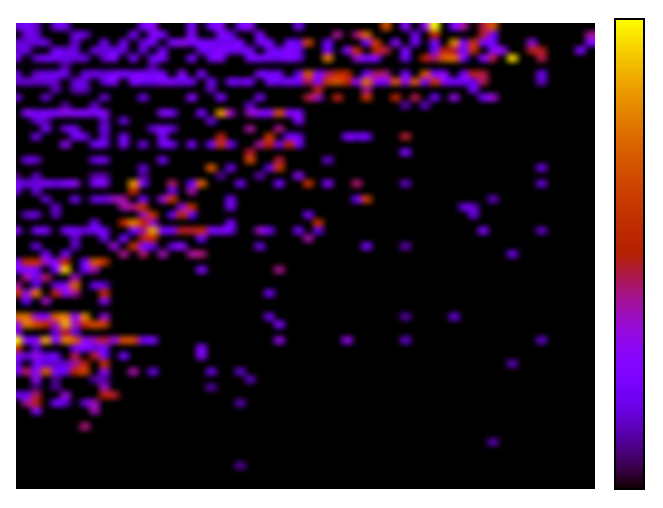
\includegraphics{IMI15}}%
    \gplfronttext
  \end{picture}%
\endgroup
} & \resizebox{0.3\textwidth}{!}{% GNUPLOT: LaTeX picture with Postscript
\begingroup
  \makeatletter
  \providecommand\color[2][]{%
    \GenericError{(gnuplot) \space\space\space\@spaces}{%
      Package color not loaded in conjunction with
      terminal option `colourtext'%
    }{See the gnuplot documentation for explanation.%
    }{Either use 'blacktext' in gnuplot or load the package
      color.sty in LaTeX.}%
    \renewcommand\color[2][]{}%
  }%
  \providecommand\includegraphics[2][]{%
    \GenericError{(gnuplot) \space\space\space\@spaces}{%
      Package graphicx or graphics not loaded%
    }{See the gnuplot documentation for explanation.%
    }{The gnuplot epslatex terminal needs graphicx.sty or graphics.sty.}%
    \renewcommand\includegraphics[2][]{}%
  }%
  \providecommand\rotatebox[2]{#2}%
  \@ifundefined{ifGPcolor}{%
    \newif\ifGPcolor
    \GPcolortrue
  }{}%
  \@ifundefined{ifGPblacktext}{%
    \newif\ifGPblacktext
    \GPblacktexttrue
  }{}%
  % define a \g@addto@macro without @ in the name:
  \let\gplgaddtomacro\g@addto@macro
  % define empty templates for all commands taking text:
  \gdef\gplbacktext{}%
  \gdef\gplfronttext{}%
  \makeatother
  \ifGPblacktext
    % no textcolor at all
    \def\colorrgb#1{}%
    \def\colorgray#1{}%
  \else
    % gray or color?
    \ifGPcolor
      \def\colorrgb#1{\color[rgb]{#1}}%
      \def\colorgray#1{\color[gray]{#1}}%
      \expandafter\def\csname LTw\endcsname{\color{white}}%
      \expandafter\def\csname LTb\endcsname{\color{black}}%
      \expandafter\def\csname LTa\endcsname{\color{black}}%
      \expandafter\def\csname LT0\endcsname{\color[rgb]{1,0,0}}%
      \expandafter\def\csname LT1\endcsname{\color[rgb]{0,1,0}}%
      \expandafter\def\csname LT2\endcsname{\color[rgb]{0,0,1}}%
      \expandafter\def\csname LT3\endcsname{\color[rgb]{1,0,1}}%
      \expandafter\def\csname LT4\endcsname{\color[rgb]{0,1,1}}%
      \expandafter\def\csname LT5\endcsname{\color[rgb]{1,1,0}}%
      \expandafter\def\csname LT6\endcsname{\color[rgb]{0,0,0}}%
      \expandafter\def\csname LT7\endcsname{\color[rgb]{1,0.3,0}}%
      \expandafter\def\csname LT8\endcsname{\color[rgb]{0.5,0.5,0.5}}%
    \else
      % gray
      \def\colorrgb#1{\color{black}}%
      \def\colorgray#1{\color[gray]{#1}}%
      \expandafter\def\csname LTw\endcsname{\color{white}}%
      \expandafter\def\csname LTb\endcsname{\color{black}}%
      \expandafter\def\csname LTa\endcsname{\color{black}}%
      \expandafter\def\csname LT0\endcsname{\color{black}}%
      \expandafter\def\csname LT1\endcsname{\color{black}}%
      \expandafter\def\csname LT2\endcsname{\color{black}}%
      \expandafter\def\csname LT3\endcsname{\color{black}}%
      \expandafter\def\csname LT4\endcsname{\color{black}}%
      \expandafter\def\csname LT5\endcsname{\color{black}}%
      \expandafter\def\csname LT6\endcsname{\color{black}}%
      \expandafter\def\csname LT7\endcsname{\color{black}}%
      \expandafter\def\csname LT8\endcsname{\color{black}}%
    \fi
  \fi
  \setlength{\unitlength}{0.0500bp}%
  \begin{picture}(7200.00,5040.00)%
    \gplgaddtomacro\gplbacktext{%
      \csname LTb\endcsname%
      \put(594,503){\makebox(0,0)[r]{\strut{} 0}}%
      \put(594,1215){\makebox(0,0)[r]{\strut{} 10}}%
      \put(594,1927){\makebox(0,0)[r]{\strut{} 20}}%
      \put(594,2639){\makebox(0,0)[r]{\strut{} 30}}%
      \put(594,3351){\makebox(0,0)[r]{\strut{} 40}}%
      \put(594,4063){\makebox(0,0)[r]{\strut{} 50}}%
      \put(594,4775){\makebox(0,0)[r]{\strut{} 60}}%
      \put(789,220){\makebox(0,0){\strut{} 0}}%
      \put(1623,220){\makebox(0,0){\strut{} 10}}%
      \put(2457,220){\makebox(0,0){\strut{} 20}}%
      \put(3291,220){\makebox(0,0){\strut{} 30}}%
      \put(4124,220){\makebox(0,0){\strut{} 40}}%
      \put(4958,220){\makebox(0,0){\strut{} 50}}%
      \put(5792,220){\makebox(0,0){\strut{} 60}}%
    }%
    \gplgaddtomacro\gplfronttext{%
      \csname LTb\endcsname%
      \put(6362,503){\makebox(0,0)[l]{\strut{} 0}}%
      \put(6362,977){\makebox(0,0)[l]{\strut{} 0.01}}%
      \put(6362,1452){\makebox(0,0)[l]{\strut{} 0.02}}%
      \put(6362,1927){\makebox(0,0)[l]{\strut{} 0.03}}%
      \put(6362,2401){\makebox(0,0)[l]{\strut{} 0.04}}%
      \put(6362,2876){\makebox(0,0)[l]{\strut{} 0.05}}%
      \put(6362,3351){\makebox(0,0)[l]{\strut{} 0.06}}%
      \put(6362,3825){\makebox(0,0)[l]{\strut{} 0.07}}%
      \put(6362,4300){\makebox(0,0)[l]{\strut{} 0.08}}%
      \put(6362,4775){\makebox(0,0)[l]{\strut{} 0.09}}%
    }%
    \gplbacktext
    \put(0,0){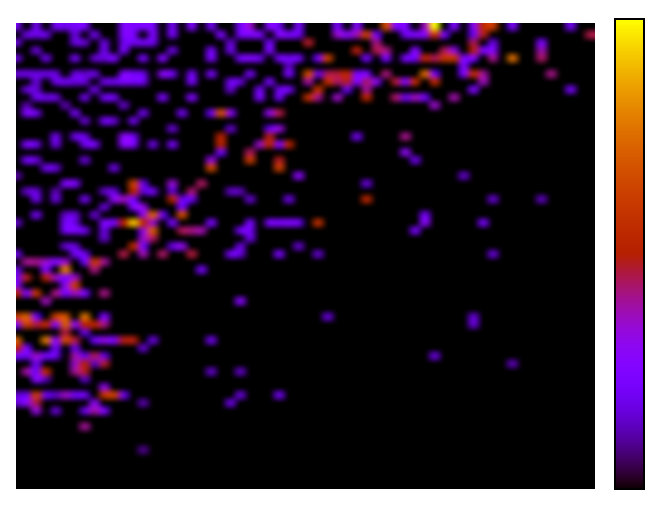
\includegraphics{IMI17}}%
    \gplfronttext
  \end{picture}%
\endgroup
} 
\end{tabular}
\bigskip
\rule{35em}{0.5pt}
\caption{\label{imires} Above are shown the peak IMI values between neurons, calculated from their spikes trains. The adjacency matrix is directed so that the peak IMI dictates the direction of influence of the neurons. The amplitude of the individual neurons in the Poisson noise layer increased from {\bf (a)} $1$ mV to {\bf (ix)}$16$ mV in steps of $2$ mV. Note that the IMI actually becomes more discriminating as the noise level increases.}
\end{center}
\end{figure}


As can be seen in figure \ref{imires}, the IMI actually improves its discriminability as the noise level increases.  This should not be a surprise, as this was the reasoning provided by the authors of \citep{SinghLesica2010a} for conditioning for the future along with the past, as opposed to just conditioning for the past as\citet{Schreiber2000a} does with the Transfer Entropy measure.  This means that the IMI could be a very good tool to measure influence between neurons in simultaneous recordings, but it does require a lot of data before it is useful, and it has a formidable calculation time.

The next step in the process is to calculate the bibliographic coupling from the thresholded adjacency matrix, $\mathbf{A}_{\tau_I}$, calculated in equation \ref{adjmat} .  This then gives a new network, which is undirected, and hence can be clustered using common methods such as \citep{Newman2006a, NewmanGirvan2004a}. 

\begin{figure}[htb]
\begin{center}
\begin{tabular}{ll}
{\bf (a)} & {\bf (b)}\\
\resizebox{0.45\textwidth}{!}{% GNUPLOT: LaTeX picture with Postscript
\begingroup
  \makeatletter
  \providecommand\color[2][]{%
    \GenericError{(gnuplot) \space\space\space\@spaces}{%
      Package color not loaded in conjunction with
      terminal option `colourtext'%
    }{See the gnuplot documentation for explanation.%
    }{Either use 'blacktext' in gnuplot or load the package
      color.sty in LaTeX.}%
    \renewcommand\color[2][]{}%
  }%
  \providecommand\includegraphics[2][]{%
    \GenericError{(gnuplot) \space\space\space\@spaces}{%
      Package graphicx or graphics not loaded%
    }{See the gnuplot documentation for explanation.%
    }{The gnuplot epslatex terminal needs graphicx.sty or graphics.sty.}%
    \renewcommand\includegraphics[2][]{}%
  }%
  \providecommand\rotatebox[2]{#2}%
  \@ifundefined{ifGPcolor}{%
    \newif\ifGPcolor
    \GPcolortrue
  }{}%
  \@ifundefined{ifGPblacktext}{%
    \newif\ifGPblacktext
    \GPblacktexttrue
  }{}%
  % define a \g@addto@macro without @ in the name:
  \let\gplgaddtomacro\g@addto@macro
  % define empty templates for all commands taking text:
  \gdef\gplbacktext{}%
  \gdef\gplfronttext{}%
  \makeatother
  \ifGPblacktext
    % no textcolor at all
    \def\colorrgb#1{}%
    \def\colorgray#1{}%
  \else
    % gray or color?
    \ifGPcolor
      \def\colorrgb#1{\color[rgb]{#1}}%
      \def\colorgray#1{\color[gray]{#1}}%
      \expandafter\def\csname LTw\endcsname{\color{white}}%
      \expandafter\def\csname LTb\endcsname{\color{black}}%
      \expandafter\def\csname LTa\endcsname{\color{black}}%
      \expandafter\def\csname LT0\endcsname{\color[rgb]{1,0,0}}%
      \expandafter\def\csname LT1\endcsname{\color[rgb]{0,1,0}}%
      \expandafter\def\csname LT2\endcsname{\color[rgb]{0,0,1}}%
      \expandafter\def\csname LT3\endcsname{\color[rgb]{1,0,1}}%
      \expandafter\def\csname LT4\endcsname{\color[rgb]{0,1,1}}%
      \expandafter\def\csname LT5\endcsname{\color[rgb]{1,1,0}}%
      \expandafter\def\csname LT6\endcsname{\color[rgb]{0,0,0}}%
      \expandafter\def\csname LT7\endcsname{\color[rgb]{1,0.3,0}}%
      \expandafter\def\csname LT8\endcsname{\color[rgb]{0.5,0.5,0.5}}%
    \else
      % gray
      \def\colorrgb#1{\color{black}}%
      \def\colorgray#1{\color[gray]{#1}}%
      \expandafter\def\csname LTw\endcsname{\color{white}}%
      \expandafter\def\csname LTb\endcsname{\color{black}}%
      \expandafter\def\csname LTa\endcsname{\color{black}}%
      \expandafter\def\csname LT0\endcsname{\color{black}}%
      \expandafter\def\csname LT1\endcsname{\color{black}}%
      \expandafter\def\csname LT2\endcsname{\color{black}}%
      \expandafter\def\csname LT3\endcsname{\color{black}}%
      \expandafter\def\csname LT4\endcsname{\color{black}}%
      \expandafter\def\csname LT5\endcsname{\color{black}}%
      \expandafter\def\csname LT6\endcsname{\color{black}}%
      \expandafter\def\csname LT7\endcsname{\color{black}}%
      \expandafter\def\csname LT8\endcsname{\color{black}}%
    \fi
  \fi
  \setlength{\unitlength}{0.0500bp}%
  \begin{picture}(7200.00,5040.00)%
    \gplgaddtomacro\gplbacktext{%
      \csname LTb\endcsname%
      \put(594,503){\makebox(0,0)[r]{\strut{} 0}}%
      \put(594,1215){\makebox(0,0)[r]{\strut{} 10}}%
      \put(594,1927){\makebox(0,0)[r]{\strut{} 20}}%
      \put(594,2639){\makebox(0,0)[r]{\strut{} 30}}%
      \put(594,3351){\makebox(0,0)[r]{\strut{} 40}}%
      \put(594,4063){\makebox(0,0)[r]{\strut{} 50}}%
      \put(594,4775){\makebox(0,0)[r]{\strut{} 60}}%
      \put(789,220){\makebox(0,0){\strut{} 0}}%
      \put(1623,220){\makebox(0,0){\strut{} 10}}%
      \put(2457,220){\makebox(0,0){\strut{} 20}}%
      \put(3291,220){\makebox(0,0){\strut{} 30}}%
      \put(4124,220){\makebox(0,0){\strut{} 40}}%
      \put(4958,220){\makebox(0,0){\strut{} 50}}%
      \put(5792,220){\makebox(0,0){\strut{} 60}}%
    }%
    \gplgaddtomacro\gplfronttext{%
      \csname LTb\endcsname%
      \put(6362,503){\makebox(0,0)[l]{\strut{} 0}}%
      \put(6362,1215){\makebox(0,0)[l]{\strut{} 5}}%
      \put(6362,1927){\makebox(0,0)[l]{\strut{} 10}}%
      \put(6362,2639){\makebox(0,0)[l]{\strut{} 15}}%
      \put(6362,3351){\makebox(0,0)[l]{\strut{} 20}}%
      \put(6362,4063){\makebox(0,0)[l]{\strut{} 25}}%
      \put(6362,4775){\makebox(0,0)[l]{\strut{} 30}}%
    }%
    \gplbacktext
    \put(0,0){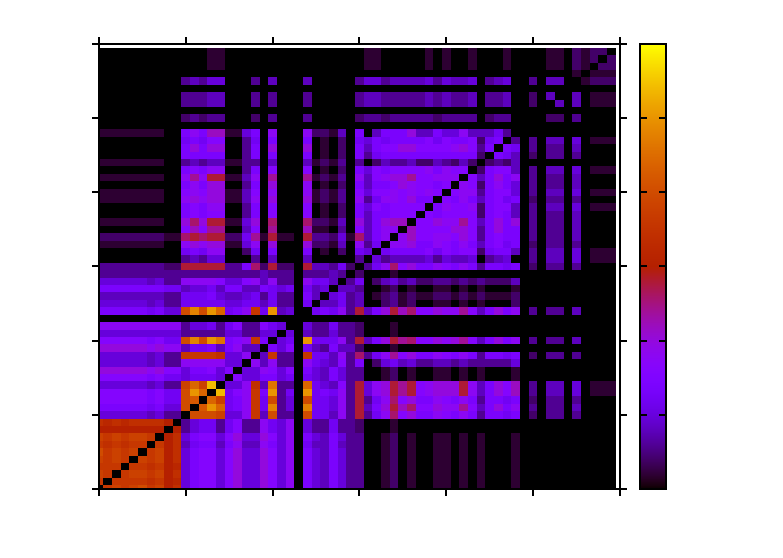
\includegraphics{TB1}}%
    \gplfronttext
  \end{picture}%
\endgroup
} & \resizebox{0.45\textwidth}{!}{% GNUPLOT: LaTeX picture with Postscript
\begingroup
  \makeatletter
  \providecommand\color[2][]{%
    \GenericError{(gnuplot) \space\space\space\@spaces}{%
      Package color not loaded in conjunction with
      terminal option `colourtext'%
    }{See the gnuplot documentation for explanation.%
    }{Either use 'blacktext' in gnuplot or load the package
      color.sty in LaTeX.}%
    \renewcommand\color[2][]{}%
  }%
  \providecommand\includegraphics[2][]{%
    \GenericError{(gnuplot) \space\space\space\@spaces}{%
      Package graphicx or graphics not loaded%
    }{See the gnuplot documentation for explanation.%
    }{The gnuplot epslatex terminal needs graphicx.sty or graphics.sty.}%
    \renewcommand\includegraphics[2][]{}%
  }%
  \providecommand\rotatebox[2]{#2}%
  \@ifundefined{ifGPcolor}{%
    \newif\ifGPcolor
    \GPcolortrue
  }{}%
  \@ifundefined{ifGPblacktext}{%
    \newif\ifGPblacktext
    \GPblacktexttrue
  }{}%
  % define a \g@addto@macro without @ in the name:
  \let\gplgaddtomacro\g@addto@macro
  % define empty templates for all commands taking text:
  \gdef\gplbacktext{}%
  \gdef\gplfronttext{}%
  \makeatother
  \ifGPblacktext
    % no textcolor at all
    \def\colorrgb#1{}%
    \def\colorgray#1{}%
  \else
    % gray or color?
    \ifGPcolor
      \def\colorrgb#1{\color[rgb]{#1}}%
      \def\colorgray#1{\color[gray]{#1}}%
      \expandafter\def\csname LTw\endcsname{\color{white}}%
      \expandafter\def\csname LTb\endcsname{\color{black}}%
      \expandafter\def\csname LTa\endcsname{\color{black}}%
      \expandafter\def\csname LT0\endcsname{\color[rgb]{1,0,0}}%
      \expandafter\def\csname LT1\endcsname{\color[rgb]{0,1,0}}%
      \expandafter\def\csname LT2\endcsname{\color[rgb]{0,0,1}}%
      \expandafter\def\csname LT3\endcsname{\color[rgb]{1,0,1}}%
      \expandafter\def\csname LT4\endcsname{\color[rgb]{0,1,1}}%
      \expandafter\def\csname LT5\endcsname{\color[rgb]{1,1,0}}%
      \expandafter\def\csname LT6\endcsname{\color[rgb]{0,0,0}}%
      \expandafter\def\csname LT7\endcsname{\color[rgb]{1,0.3,0}}%
      \expandafter\def\csname LT8\endcsname{\color[rgb]{0.5,0.5,0.5}}%
    \else
      % gray
      \def\colorrgb#1{\color{black}}%
      \def\colorgray#1{\color[gray]{#1}}%
      \expandafter\def\csname LTw\endcsname{\color{white}}%
      \expandafter\def\csname LTb\endcsname{\color{black}}%
      \expandafter\def\csname LTa\endcsname{\color{black}}%
      \expandafter\def\csname LT0\endcsname{\color{black}}%
      \expandafter\def\csname LT1\endcsname{\color{black}}%
      \expandafter\def\csname LT2\endcsname{\color{black}}%
      \expandafter\def\csname LT3\endcsname{\color{black}}%
      \expandafter\def\csname LT4\endcsname{\color{black}}%
      \expandafter\def\csname LT5\endcsname{\color{black}}%
      \expandafter\def\csname LT6\endcsname{\color{black}}%
      \expandafter\def\csname LT7\endcsname{\color{black}}%
      \expandafter\def\csname LT8\endcsname{\color{black}}%
    \fi
  \fi
  \setlength{\unitlength}{0.0500bp}%
  \begin{picture}(7200.00,5040.00)%
    \gplgaddtomacro\gplbacktext{%
      \csname LTb\endcsname%
      \put(594,503){\makebox(0,0)[r]{\strut{} 0}}%
      \put(594,1215){\makebox(0,0)[r]{\strut{} 10}}%
      \put(594,1927){\makebox(0,0)[r]{\strut{} 20}}%
      \put(594,2639){\makebox(0,0)[r]{\strut{} 30}}%
      \put(594,3351){\makebox(0,0)[r]{\strut{} 40}}%
      \put(594,4063){\makebox(0,0)[r]{\strut{} 50}}%
      \put(594,4775){\makebox(0,0)[r]{\strut{} 60}}%
      \put(789,220){\makebox(0,0){\strut{} 0}}%
      \put(1623,220){\makebox(0,0){\strut{} 10}}%
      \put(2457,220){\makebox(0,0){\strut{} 20}}%
      \put(3291,220){\makebox(0,0){\strut{} 30}}%
      \put(4124,220){\makebox(0,0){\strut{} 40}}%
      \put(4958,220){\makebox(0,0){\strut{} 50}}%
      \put(5792,220){\makebox(0,0){\strut{} 60}}%
    }%
    \gplgaddtomacro\gplfronttext{%
      \csname LTb\endcsname%
      \put(6362,503){\makebox(0,0)[l]{\strut{} 0}}%
      \put(6362,1215){\makebox(0,0)[l]{\strut{} 1}}%
      \put(6362,1927){\makebox(0,0)[l]{\strut{} 2}}%
      \put(6362,2639){\makebox(0,0)[l]{\strut{} 3}}%
      \put(6362,3351){\makebox(0,0)[l]{\strut{} 4}}%
      \put(6362,4063){\makebox(0,0)[l]{\strut{} 5}}%
      \put(6362,4775){\makebox(0,0)[l]{\strut{} 6}}%
    }%
    \gplbacktext
    \put(0,0){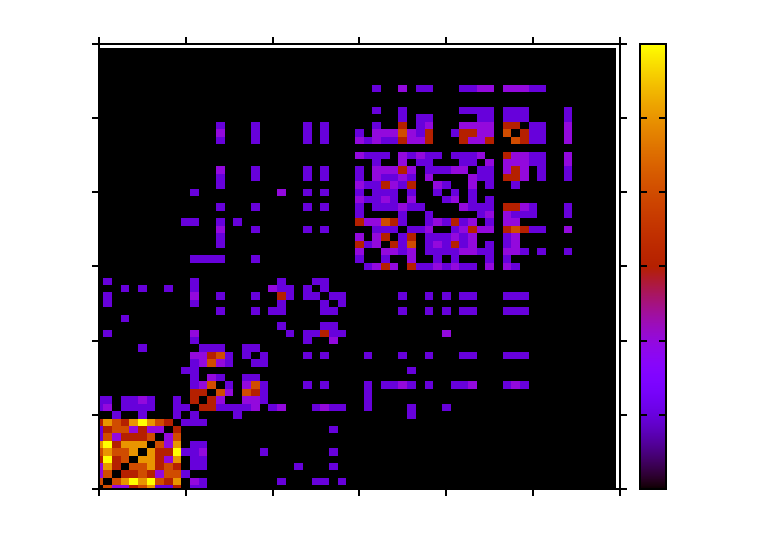
\includegraphics{TB17}}%
    \gplfronttext
  \end{picture}%
\endgroup
}
\end{tabular}
\end{center}
\bigskip
\rule{35em}{0.5pt}
\caption{\label{bibt} In this figure the thresholded bibliographic network is shown from the IMI network when: {\bf (a)} the noise level is very low, that is 1 mV from each Poisson noise neuron, and {\bf (b)} the noise level is much higher, 17mV from each Poisson neuron. The modular structure of the network is showing a lot more when the noise level is high.}
\end{figure}

In figure \ref{bibt}, the bibliographic network is shown to roughly group the first three groups together, but the fourth and fifth are also clustered together.  This is because they both influence the sixth group, so they have high bibliographic coupling.  It appears that the bibliographic coupling can detect a divergence of groups in a network, but cannot detect a convergence.

In order to correctly cluster the convergent groups towards the end of the model network, another measure needs to be introduced, the cocitation.  This coupling is similar to the bibliographic coupling, as it is the number of common nodes pointing at both nodes.  That is:
\begin{equation}
C_{ij} = \sum_k A_{ik}A{jk}
\end{equation}
The matrix is then $\mathbf{C} = \mathbf{BB}^T$.  This is another very common symmetrisation of matrices.

After running the whole process again with the cocitation instead of the bibliographic coupling, it is clear that the cocitation does indeed detect convergences in the groups of neurons.

\begin{figure}[htb]
\begin{center}
\begin{tabular}{ll}
{\bf (a)} & {\bf (b)}\\
\resizebox{0.45\textwidth}{!}{% GNUPLOT: LaTeX picture with Postscript
\begingroup
  \makeatletter
  \providecommand\color[2][]{%
    \GenericError{(gnuplot) \space\space\space\@spaces}{%
      Package color not loaded in conjunction with
      terminal option `colourtext'%
    }{See the gnuplot documentation for explanation.%
    }{Either use 'blacktext' in gnuplot or load the package
      color.sty in LaTeX.}%
    \renewcommand\color[2][]{}%
  }%
  \providecommand\includegraphics[2][]{%
    \GenericError{(gnuplot) \space\space\space\@spaces}{%
      Package graphicx or graphics not loaded%
    }{See the gnuplot documentation for explanation.%
    }{The gnuplot epslatex terminal needs graphicx.sty or graphics.sty.}%
    \renewcommand\includegraphics[2][]{}%
  }%
  \providecommand\rotatebox[2]{#2}%
  \@ifundefined{ifGPcolor}{%
    \newif\ifGPcolor
    \GPcolortrue
  }{}%
  \@ifundefined{ifGPblacktext}{%
    \newif\ifGPblacktext
    \GPblacktexttrue
  }{}%
  % define a \g@addto@macro without @ in the name:
  \let\gplgaddtomacro\g@addto@macro
  % define empty templates for all commands taking text:
  \gdef\gplbacktext{}%
  \gdef\gplfronttext{}%
  \makeatother
  \ifGPblacktext
    % no textcolor at all
    \def\colorrgb#1{}%
    \def\colorgray#1{}%
  \else
    % gray or color?
    \ifGPcolor
      \def\colorrgb#1{\color[rgb]{#1}}%
      \def\colorgray#1{\color[gray]{#1}}%
      \expandafter\def\csname LTw\endcsname{\color{white}}%
      \expandafter\def\csname LTb\endcsname{\color{black}}%
      \expandafter\def\csname LTa\endcsname{\color{black}}%
      \expandafter\def\csname LT0\endcsname{\color[rgb]{1,0,0}}%
      \expandafter\def\csname LT1\endcsname{\color[rgb]{0,1,0}}%
      \expandafter\def\csname LT2\endcsname{\color[rgb]{0,0,1}}%
      \expandafter\def\csname LT3\endcsname{\color[rgb]{1,0,1}}%
      \expandafter\def\csname LT4\endcsname{\color[rgb]{0,1,1}}%
      \expandafter\def\csname LT5\endcsname{\color[rgb]{1,1,0}}%
      \expandafter\def\csname LT6\endcsname{\color[rgb]{0,0,0}}%
      \expandafter\def\csname LT7\endcsname{\color[rgb]{1,0.3,0}}%
      \expandafter\def\csname LT8\endcsname{\color[rgb]{0.5,0.5,0.5}}%
    \else
      % gray
      \def\colorrgb#1{\color{black}}%
      \def\colorgray#1{\color[gray]{#1}}%
      \expandafter\def\csname LTw\endcsname{\color{white}}%
      \expandafter\def\csname LTb\endcsname{\color{black}}%
      \expandafter\def\csname LTa\endcsname{\color{black}}%
      \expandafter\def\csname LT0\endcsname{\color{black}}%
      \expandafter\def\csname LT1\endcsname{\color{black}}%
      \expandafter\def\csname LT2\endcsname{\color{black}}%
      \expandafter\def\csname LT3\endcsname{\color{black}}%
      \expandafter\def\csname LT4\endcsname{\color{black}}%
      \expandafter\def\csname LT5\endcsname{\color{black}}%
      \expandafter\def\csname LT6\endcsname{\color{black}}%
      \expandafter\def\csname LT7\endcsname{\color{black}}%
      \expandafter\def\csname LT8\endcsname{\color{black}}%
    \fi
  \fi
  \setlength{\unitlength}{0.0500bp}%
  \begin{picture}(7200.00,5040.00)%
    \gplgaddtomacro\gplbacktext{%
      \csname LTb\endcsname%
      \put(594,503){\makebox(0,0)[r]{\strut{} 0}}%
      \put(594,1215){\makebox(0,0)[r]{\strut{} 10}}%
      \put(594,1927){\makebox(0,0)[r]{\strut{} 20}}%
      \put(594,2639){\makebox(0,0)[r]{\strut{} 30}}%
      \put(594,3351){\makebox(0,0)[r]{\strut{} 40}}%
      \put(594,4063){\makebox(0,0)[r]{\strut{} 50}}%
      \put(594,4775){\makebox(0,0)[r]{\strut{} 60}}%
      \put(789,220){\makebox(0,0){\strut{} 0}}%
      \put(1623,220){\makebox(0,0){\strut{} 10}}%
      \put(2457,220){\makebox(0,0){\strut{} 20}}%
      \put(3291,220){\makebox(0,0){\strut{} 30}}%
      \put(4124,220){\makebox(0,0){\strut{} 40}}%
      \put(4958,220){\makebox(0,0){\strut{} 50}}%
      \put(5792,220){\makebox(0,0){\strut{} 60}}%
    }%
    \gplgaddtomacro\gplfronttext{%
      \csname LTb\endcsname%
      \put(6362,503){\makebox(0,0)[l]{\strut{} 0}}%
      \put(6362,1215){\makebox(0,0)[l]{\strut{} 5}}%
      \put(6362,1927){\makebox(0,0)[l]{\strut{} 10}}%
      \put(6362,2639){\makebox(0,0)[l]{\strut{} 15}}%
      \put(6362,3351){\makebox(0,0)[l]{\strut{} 20}}%
      \put(6362,4063){\makebox(0,0)[l]{\strut{} 25}}%
      \put(6362,4775){\makebox(0,0)[l]{\strut{} 30}}%
    }%
    \gplbacktext
    \put(0,0){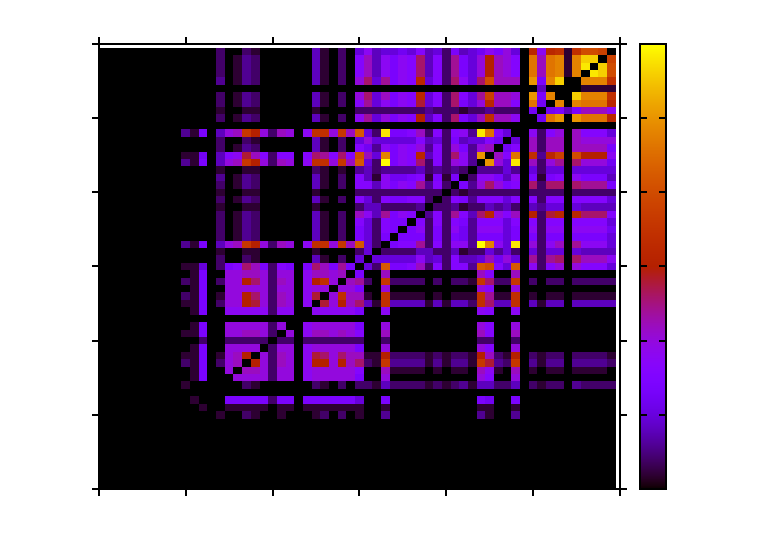
\includegraphics{TC1}}%
    \gplfronttext
  \end{picture}%
\endgroup
} & \resizebox{0.45\textwidth}{!}{% GNUPLOT: LaTeX picture with Postscript
\begingroup
  \makeatletter
  \providecommand\color[2][]{%
    \GenericError{(gnuplot) \space\space\space\@spaces}{%
      Package color not loaded in conjunction with
      terminal option `colourtext'%
    }{See the gnuplot documentation for explanation.%
    }{Either use 'blacktext' in gnuplot or load the package
      color.sty in LaTeX.}%
    \renewcommand\color[2][]{}%
  }%
  \providecommand\includegraphics[2][]{%
    \GenericError{(gnuplot) \space\space\space\@spaces}{%
      Package graphicx or graphics not loaded%
    }{See the gnuplot documentation for explanation.%
    }{The gnuplot epslatex terminal needs graphicx.sty or graphics.sty.}%
    \renewcommand\includegraphics[2][]{}%
  }%
  \providecommand\rotatebox[2]{#2}%
  \@ifundefined{ifGPcolor}{%
    \newif\ifGPcolor
    \GPcolortrue
  }{}%
  \@ifundefined{ifGPblacktext}{%
    \newif\ifGPblacktext
    \GPblacktexttrue
  }{}%
  % define a \g@addto@macro without @ in the name:
  \let\gplgaddtomacro\g@addto@macro
  % define empty templates for all commands taking text:
  \gdef\gplbacktext{}%
  \gdef\gplfronttext{}%
  \makeatother
  \ifGPblacktext
    % no textcolor at all
    \def\colorrgb#1{}%
    \def\colorgray#1{}%
  \else
    % gray or color?
    \ifGPcolor
      \def\colorrgb#1{\color[rgb]{#1}}%
      \def\colorgray#1{\color[gray]{#1}}%
      \expandafter\def\csname LTw\endcsname{\color{white}}%
      \expandafter\def\csname LTb\endcsname{\color{black}}%
      \expandafter\def\csname LTa\endcsname{\color{black}}%
      \expandafter\def\csname LT0\endcsname{\color[rgb]{1,0,0}}%
      \expandafter\def\csname LT1\endcsname{\color[rgb]{0,1,0}}%
      \expandafter\def\csname LT2\endcsname{\color[rgb]{0,0,1}}%
      \expandafter\def\csname LT3\endcsname{\color[rgb]{1,0,1}}%
      \expandafter\def\csname LT4\endcsname{\color[rgb]{0,1,1}}%
      \expandafter\def\csname LT5\endcsname{\color[rgb]{1,1,0}}%
      \expandafter\def\csname LT6\endcsname{\color[rgb]{0,0,0}}%
      \expandafter\def\csname LT7\endcsname{\color[rgb]{1,0.3,0}}%
      \expandafter\def\csname LT8\endcsname{\color[rgb]{0.5,0.5,0.5}}%
    \else
      % gray
      \def\colorrgb#1{\color{black}}%
      \def\colorgray#1{\color[gray]{#1}}%
      \expandafter\def\csname LTw\endcsname{\color{white}}%
      \expandafter\def\csname LTb\endcsname{\color{black}}%
      \expandafter\def\csname LTa\endcsname{\color{black}}%
      \expandafter\def\csname LT0\endcsname{\color{black}}%
      \expandafter\def\csname LT1\endcsname{\color{black}}%
      \expandafter\def\csname LT2\endcsname{\color{black}}%
      \expandafter\def\csname LT3\endcsname{\color{black}}%
      \expandafter\def\csname LT4\endcsname{\color{black}}%
      \expandafter\def\csname LT5\endcsname{\color{black}}%
      \expandafter\def\csname LT6\endcsname{\color{black}}%
      \expandafter\def\csname LT7\endcsname{\color{black}}%
      \expandafter\def\csname LT8\endcsname{\color{black}}%
    \fi
  \fi
  \setlength{\unitlength}{0.0500bp}%
  \begin{picture}(7200.00,5040.00)%
    \gplgaddtomacro\gplbacktext{%
      \csname LTb\endcsname%
      \put(594,503){\makebox(0,0)[r]{\strut{} 0}}%
      \put(594,1215){\makebox(0,0)[r]{\strut{} 10}}%
      \put(594,1927){\makebox(0,0)[r]{\strut{} 20}}%
      \put(594,2639){\makebox(0,0)[r]{\strut{} 30}}%
      \put(594,3351){\makebox(0,0)[r]{\strut{} 40}}%
      \put(594,4063){\makebox(0,0)[r]{\strut{} 50}}%
      \put(594,4775){\makebox(0,0)[r]{\strut{} 60}}%
      \put(789,220){\makebox(0,0){\strut{} 0}}%
      \put(1623,220){\makebox(0,0){\strut{} 10}}%
      \put(2457,220){\makebox(0,0){\strut{} 20}}%
      \put(3291,220){\makebox(0,0){\strut{} 30}}%
      \put(4124,220){\makebox(0,0){\strut{} 40}}%
      \put(4958,220){\makebox(0,0){\strut{} 50}}%
      \put(5792,220){\makebox(0,0){\strut{} 60}}%
    }%
    \gplgaddtomacro\gplfronttext{%
      \csname LTb\endcsname%
      \put(6362,503){\makebox(0,0)[l]{\strut{} 0}}%
      \put(6362,1037){\makebox(0,0)[l]{\strut{} 1}}%
      \put(6362,1571){\makebox(0,0)[l]{\strut{} 2}}%
      \put(6362,2105){\makebox(0,0)[l]{\strut{} 3}}%
      \put(6362,2639){\makebox(0,0)[l]{\strut{} 4}}%
      \put(6362,3173){\makebox(0,0)[l]{\strut{} 5}}%
      \put(6362,3707){\makebox(0,0)[l]{\strut{} 6}}%
      \put(6362,4241){\makebox(0,0)[l]{\strut{} 7}}%
      \put(6362,4775){\makebox(0,0)[l]{\strut{} 8}}%
    }%
    \gplbacktext
    \put(0,0){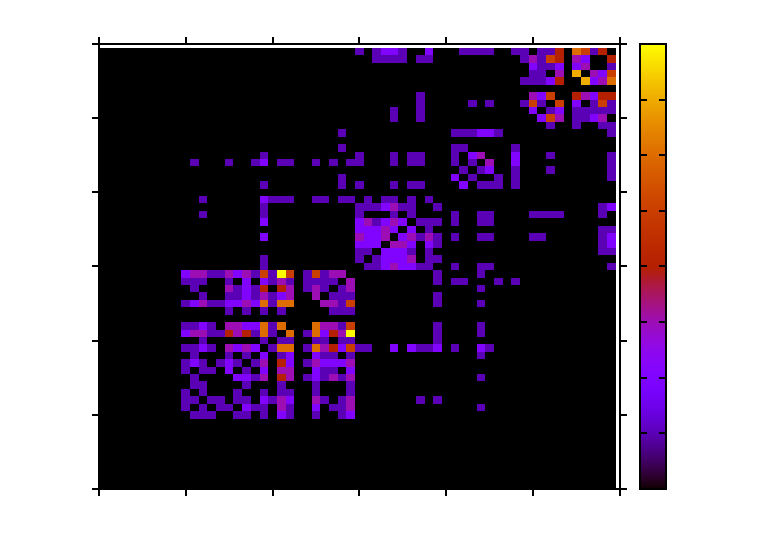
\includegraphics{TC17}}%
    \gplfronttext
  \end{picture}%
\endgroup
}
\end{tabular}
\end{center}
\bigskip
\rule{35em}{0.5pt}
\caption{\label{cocitt} In this figure the thresholded cocitation network is shown from  the IMI network when: {\bf (a)} the noise level is very low, that is 1 mV from each Poisson noise neuron, and {\bf (b)} the noise level is much higher, 17mV from each Poisson neuron. The modular structure of the network is showing a lot more when the noise level is high.}
\end{figure}

\section{Spike timing dependent plasticity}
\citet{SongEtAl2000a} introduced a plasticity rule for synapses in artificial networks which led to a stable, more energy-efficient communication to be learned.  The rule is simply based on the temporal order of neuronal spiking.

If neuron $B$ spikes soon after neuron $A$, then the synapse from $A$ to $B$ is strengthened, but the synapse from $B$ to $A$ is weakened.  This leads to neurons which spike together to do so more, and pathways form within the network. The mathematical formula for spike-timing dependent plasticity (STDP) is:
%\begin{equation}
%
%\end{equation}


\section{Discussion}
Two new algorithms were introduced to try to find a clustering that would maximise the modularity of a network. Neither produced results better than the standard methods, so were used sparingly.  The simulated annealing algorithm appeared to not necessarily maximise the modularity, but seemed to find the highest \lq{}stable\rq{} modularity. 

Network methods did not cluster stimuli well, perhaps because the network structure was not natural.  Perhaps the simulated annealing algorithm introduce in this chapter could provide interesting clusterings of stimuli.

The incremental mutual information proved to be a remarkably useful tool in noisy networks, but it requires very long data sets to calculate.  The length of data sets required may rule out the IMI as a useful measure of real world data.

The bibliographic coupling and  the cocitation both gave interesting clusterings of the network, but combining them proved to be a difficult task.
